%% Pattern Recognition submission.
%% GENERATED by tools/make_pr_tex.py from main.tex -- edit that, not this.
%%
%% `review` gives what Elsevier asks for at submission: one column, double
%% spacing, line numbers.  Use [preprint,12pt] for a compact reading copy, or
%% [final,5p,times] once the paper is accepted.
%% PR asks for single column, double spaced, Times New Roman, 10pt including
%% tables.  `review` gives the column and the spacing, `times` the face,
%% `10pt` the size.
\documentclass[review,10pt,times]{elsarticle}

% PR's journal-specific section asks for margins of 4.3cm, 4.8cm, 4.3cm,
% 4.8cm (top, right, bottom, left).  Those only add up on A4; elsarticle
% defaults to US Letter with its own margins, so both are set here.  The
% resulting text block is 322pt, narrower than the 345pt the class gives,
% which is why the \fitbox tables and the two \makebox figures matter.
\usepackage[a4paper,top=4.3cm,right=4.8cm,bottom=4.3cm,left=4.8cm]{geometry}

\usepackage[T1]{fontenc}

\usepackage{graphicx}
\usepackage{tikz}                  % two figures are drawn, not imported
\usetikzlibrary{arrows.meta,positioning,fit,backgrounds,calc}
% Colours and node styles shared by the drawn figures (fig_ladder_tikz,
% fig_method_tikz).  Input from the preamble so both builds agree.
%
% The palette is deliberately narrow -- two hues carry the two regions, one
% carries the adapter, one marks the injection sites -- and every stroke/fill
% pair stays distinguishable in greyscale, since reviewers print in black and
% white.  Nothing is distinguished by colour alone; every element is labelled.

\definecolor{fgBlue}{HTML}{2F6FB0}
\definecolor{fgGreen}{HTML}{3AA66A}
\definecolor{fgOrange}{HTML}{D9862B}
\definecolor{fgPurple}{HTML}{7A5AA6}
\definecolor{fgRed}{HTML}{B94040}
\definecolor{fgGrey}{HTML}{6B6B6B}
\definecolor{bgBlue}{HTML}{EAF1F8}
\definecolor{bgGreen}{HTML}{E9F5EE}
\definecolor{bgOrange}{HTML}{FBF0DD}
\definecolor{bgPurple}{HTML}{F0EBF6}
\definecolor{bgGrey}{HTML}{F4F4F4}
% Stage bands sit behind everything and must stay very light, or they compete
% with the boxes on top of them.
\definecolor{bandA}{HTML}{F7F9FC}
\definecolor{bandB}{HTML}{FAF7F4}
\definecolor{rule}{HTML}{D8DCE2}

\tikzset{
  blk/.style     = {draw=fgGrey!80, fill=white, rounded corners=1.6pt,
                    align=center, inner sep=2.6pt, font=\scriptsize,
                    line width=0.5pt},
  blkb/.style    = {blk, draw=fgBlue,   fill=bgBlue},
  blkg/.style    = {blk, draw=fgGreen,  fill=bgGreen},
  blko/.style    = {blk, draw=fgOrange, fill=bgOrange},
  blkp/.style    = {blk, draw=fgPurple, fill=bgPurple},
  blkr/.style    = {blk, draw=fgRed,    fill=white},
  ar/.style      = {-{Stealth[length=3.4pt,width=2.6pt]}, draw=fgGrey,
                    line width=0.45pt},
  arh/.style     = {ar, draw=black, line width=0.6pt},
  % A numbered injection-site marker.
  site/.style    = {circle, draw=fgRed, fill=white, text=fgRed, inner sep=0pt,
                    minimum size=8pt, font=\scriptsize\bfseries,
                    line width=0.5pt},
  lbl/.style     = {font=\scriptsize, text=black, align=center, inner sep=1pt},
  slbl/.style    = {font=\tiny, text=fgGrey, align=center, inner sep=1pt},
  stage/.style   = {font=\scriptsize\bfseries, text=black, align=left,
                    inner sep=0pt},
  band/.style    = {rounded corners=2.5pt, draw=rule, line width=0.4pt},
  % A thumbnail of a real render, so the diagram is anchored to what the
  % method actually produces rather than to coloured rectangles.
  thumb/.style   = {inner sep=0pt, outer sep=0pt, draw=fgGrey!60,
                    line width=0.4pt},
}

% Frozen marker.  Every module in this method is frozen -- no diffusion model,
% adapter or text encoder is fine-tuned -- which is the point, so it is worth
% a glyph rather than a sentence.  Drawn rather than taken from a symbol font
% so it survives any font setup.
\newcommand{\frozen}[1][0.9]{%
  \tikz[baseline=-0.55ex,scale=#1]{%
    \foreach \a in {0,60,120}{%
      \draw[fgBlue,line width=0.35pt] (\a:2.1pt) -- (\a+180:2.1pt);}
    \foreach \a in {0,60,120,180,240,300}{%
      \draw[fgBlue,line width=0.35pt] (\a:2.1pt) -- ++(\a+140:0.8pt);
      \draw[fgBlue,line width=0.35pt] (\a:2.1pt) -- ++(\a-140:0.8pt);}}}

\usepackage[export]{adjustbox}     % max width/height keys for \includegraphics
\usepackage[htt]{hyphenat}         % long \texttt weight names may hyphenate
\usepackage{amsmath}
\usepackage{amssymb}
\usepackage{booktabs}
\usepackage{multirow}
\usepackage{xcolor}
\usepackage{microtype}
\usepackage{float}
\usepackage{xspace}
\usepackage{setspace}
\usepackage{etoolbox}
% Elsevier asks the review copy to carry continuous line numbers, and this
% elsarticle's `review` option does not load lineno itself.
\usepackage{lineno}
% PR asks for footnotes and captions at 8pt against 10pt text, which is
% \footnotesize here.  singlelinecheck measures a whole caption as one line to
% decide whether to centre it; on captions this long that overflows TeX's
% largest dimension, so it is off.
\usepackage[font=footnotesize,labelfont=bf,singlelinecheck=false]{caption}
% Each document cites the other; xr reads the other's .aux.  Build order is
% main, supp, main, supp -- the first pass of each has nothing to read yet.
\usepackage{xr}
\externaldocument{main_pr}
\usepackage[hidelinks]{hyperref}   % last: elsarticle[review] loads lineno

% `review` double-spaces everything, table rows and captions included, which
% makes the taller tables overflow the page by ~300pt.  A table is read as a
% block rather than line by line, so keep floats single-spaced; the running
% text, which is what a reviewer annotates, stays double.
\AtBeginEnvironment{table}{\singlespacing}
\AtBeginEnvironment{figure}{\singlespacing}

% One column at 12pt leaves TeX little room to breathe around the long
% \texttt{} weight names, so let it stretch a line rather than overrun.
\setlength{\emergencystretch}{3em}

% Abbreviation macros.  The body uses these; they came from cvpr.sty.
\newcommand\eg{\emph{e.g}\onedot}
\newcommand\ie{\emph{i.e}\onedot}
\newcommand\Eg{\emph{E.g}\onedot}
\newcommand\Ie{\emph{I.e}\onedot}
\newcommand\cf{\emph{cf}\onedot}
\newcommand\etc{\emph{etc}\onedot}
\newcommand\vs{\emph{vs}\onedot}
\newcommand\wrt{w.r.t\onedot}
\newcommand\etal{\emph{et al}\onedot}
\def\onedot{.\xspace}

% Shrink a table to fit, never stretch it to fill.  The tables were sized for
% a 237pt CVPR column; \columnwidth here is half again as wide, so resizing to
% it unconditionally would scale them *up*.  Height matters too: the widest
% tables are also the tallest, and at 12pt single column several overrun the
% page.
\newcommand{\fitbox}[1]{%
  \adjustbox{max width=\linewidth,max totalheight=0.88\textheight}{#1}}

% Float placement: wide tables rarely fit the space left on a page, and [h]
% alone defers them to the final \clearpage, i.e. past the bibliography.
\renewcommand{\topfraction}{0.9}
\renewcommand{\bottomfraction}{0.8}
\renewcommand{\textfraction}{0.07}
\renewcommand{\floatpagefraction}{0.75}
\setcounter{topnumber}{3}
\setcounter{bottomnumber}{2}
\setcounter{totalnumber}{5}

% lineno stops counting at an AMS display environment unless the environment
% is wrapped in \linenomath, so the numbers would restart after every
% equation.  This is the standard patch.
\newcommand*\patchAmsMathEnvironmentForLineno[1]{%
  \expandafter\let\csname old#1\expandafter\endcsname\csname #1\endcsname
  \expandafter\let\csname oldend#1\expandafter\endcsname\csname end#1\endcsname
  \renewenvironment{#1}%
    {\linenomath\csname old#1\endcsname}%
    {\csname oldend#1\endcsname\endlinenomath}}
\newcommand*\patchBothAmsMathEnvironmentsForLineno[1]{%
  \patchAmsMathEnvironmentForLineno{#1}%
  \patchAmsMathEnvironmentForLineno{#1*}}
\AtBeginDocument{%
  \patchBothAmsMathEnvironmentsForLineno{equation}%
  \patchBothAmsMathEnvironmentsForLineno{align}%
  \patchBothAmsMathEnvironmentsForLineno{gather}%
  \patchBothAmsMathEnvironmentsForLineno{multline}}

\journal{Pattern Recognition}


% Supplementary sections, tables and figures are numbered S1, S2, ... so a
% reference cannot be confused with one into the manuscript.
\renewcommand{\thesection}{S\arabic{section}}
\renewcommand{\thetable}{S\arabic{table}}
\renewcommand{\thefigure}{S\arabic{figure}}
\renewcommand{\theequation}{S\arabic{equation}}

\begin{document}

\begin{center}
  {\large\bfseries Supplementary Material\par}
  \vspace{4pt}
  {\normalsize The Injection Site Determines What Identity Survives in
   Training-Free Multi-Concept Personalization\par}
\end{center}

\vspace{6pt}
\noindent
This document holds results that support the manuscript without carrying its
argument: per-category and per-benchmark breakdowns, the component ablation,
the scaling study, failure cases, cost, and the relation to training-based
personalisation.  Section numbers are those the manuscript cites.

\linenumbers

\section{How Conceptrol was run}
\noindent\textit{Conceptrol setup.}
\label{sec:conceptrol_setup}
We use the authors' \texttt{Conceptrol\allowbreak IPAdapter\allowbreak Plus\allowbreak XL} unmodified, on the same
SDXL-base-1.0 backbone and the same \texttt{ip-adapter-plus\_sdxl\_vit-h}
weights as our method ($16$ image tokens), at $768\!\times\!768$, 30
DPM-Solver++ steps, CFG 7.5, seed 42.  Conceptrol derives its concept masks
from text cross-attention and has no layout planner, so it receives the global
prompt and the same per-region references; this is its intended usage.  We make
one change, which favours the baseline.  Its helper locates a concept's tokens
with \texttt{tokens.index(subject\_tokens[0])}, i.e.\ the \emph{first}
occurrence, which returns overlapping or misplaced spans on 36 of our 150
prompts---the person and mixed splits routinely repeat a head noun (``a teenage
girl \ldots\ a teenage girl'').  We replace it with an ordered subsequence
search that advances a cursor past each match, giving disjoint, correctly
placed spans on all 150 prompts.  Conceptrol therefore receives better concept
indices than its own helper produces.  We also swept the injection scale over
$\{0.8, 1.0\}$ across the full benchmark and report the stronger result.

\section{How MS-Diffusion was run}
\noindent\textit{MS-Diffusion setup.}
\label{sec:msdiffusion_setup}
We run the authors' released code and \texttt{ms\_adapter.bin} on
SDXL-base-1.0 with the CLIP-G image encoder they specify, at
$768\!\times\!768$, 30 DPM-Solver++ steps, CFG 7.5, seed 42 and our negative
prompt, so the two methods differ in mechanism rather than in sampling
configuration.  Each planned region is passed as one normalised box and the
head noun phrase of its sub-prompt as the matching phrase.  Two details
favour the baseline.  Its span helper matches on whitespace-split words and
strips trailing punctuation on the prompt side only, so a phrase carrying an
internal comma silently resolves to the empty span $[0,0]$ and the layout
guidance is disabled; we verified on all 150 prompts that the phrases we pass
resolve to non-empty, mutually disjoint spans.  Adjacent full-height boxes
also leave no background region, so we additionally ran the tighter,
non-adjacent box shape used in the authors' own examples, and report the
stronger of the two.  As with the other baselines, the injection scale was
swept and the better setting reported.

\section{What the ArcFace averaging convention flatters}
\noindent\textit{ArcFace is averaged over the regions where a face was found,
and that flatters the weak rows.}
Our ArcFace columns follow the usual practice of averaging over regions in
which a detector finds a face.  A method that renders one subject instead of
two is then scored on the one it rendered, and a method that renders neither
contributes nothing to the mean---so failing to produce a subject costs
nothing.  Detection rates differ enough across methods for this to matter.  On
the 50 person samples ($115$ regions) they range from $45\%$ to $96\%$.

\begin{table}[htbp]
\centering
\caption{%
  \textbf{Reported ArcFace against the same score with missing faces counted
  as zero.}  Person samples of Mixed-Eval-v1, $115$ regions.  The ranking is
  unchanged, and the margin over every baseline widens, because the baselines
  are the ones that often render no face at all.%
}
\label{tab:detect}
\resizebox{\columnwidth}{!}{%
\begin{tabular}{lccc}
\toprule
Method & Detected & ArcFace (drop) & ArcFace (zero) \\
\midrule
IP-Adapter (global)& \phantom{0}45\% & 0.113 & 0.051 \\
RPG-only           & \phantom{0}59\% & 0.129 & 0.076 \\
Attention gating   & \phantom{0}70\% & 0.118 & 0.082 \\
IP-FaceID          & \phantom{0}74\% & 0.216 & 0.160 \\
MS-Diffusion       & \phantom{0}97\% & 0.290 & 0.280 \\
\textbf{Ours}      & \phantom{0}96\% & \textbf{0.354} & \textbf{0.339} \\
\bottomrule
\end{tabular}%
}
\end{table}

Our own score barely moves ($0.354\!\to\!0.339$) because we render a face in
$96\%$ of person regions; the text-only baseline loses $41\%$ of its score and
global injection loses $55\%$, since both frequently produce no recognisable
face for the detector to score.  The advantage over the text-only baseline
therefore grows from $2.7\times$ to $4.5\times$ under the stricter policy.  We
report the drop policy in Table~\ref{tab:main} to stay comparable with prior
work and give the zero policy here, rather than choosing the one that suits
us.

\noindent\textit{Global IP injection overwrites the layout.}
Without regional control the reference's features permeate the canvas, and the
Margin is the most negative of any method here: every region crop resembles the
\emph{wrong} reference more than its own.  Fig.~\ref{fig:teaser} shows the
mechanism---conditioned on the first reference, the model renders that subject
across the whole frame and the second concept is absent.  Prompt adherence and
per-region face identity fall with it, and identity specificity falls to
$0.076$, \emph{below} the $0.082$ of a text-only run that never sees a
reference at all: the second region's crop now matches a distractor.

\noindent\textit{Conceptrol writes identity but does not separate the
concepts.}
Run from the authors' code, Conceptrol beats both text-only regional
diffusion and global injection on the identity axes: its attention-derived
masks do transfer appearance.  What it does not do is keep the concepts apart.
Its Margin is $+0.004$---each region crop is as similar to the reference it was
\emph{not} assigned as to the one it was---because given a two-subject prompt
it typically renders a \emph{single} merged subject carrying attributes of
both, rather than two subjects in two places (Supplementary~S5).  That also
explains its low prompt adherence: one merged subject does not satisfy a
prompt naming a left and a right one.  Our method reaches Margin $+0.488$ on
the same inputs, with DINO-ID $1.9\times$ and ArcFace $1.7\times$ higher.

\section{Why FID and KID rank these methods backwards}
\noindent\textit{Both distributional metrics reward failing the task.}
We report FID and KID and rely on neither, because the ordering they produce
is structural.  The reference distribution is the 750 Mixed-Eval-v1 reference
photographs, each showing a \emph{single} subject, while every method is asked
for \emph{two or three} in one frame.  No method that performs the task can
match that distribution; the way to score well is to render one clean, centred
subject.  Global IP-Adapter does exactly that, taking the best FID and KID
while having the worst Margin, the lowest CLIP-T, and only one of the two
requested concepts present---half the task missing is invisible to both
metrics.  Conceptrol is second on both for the same reason.

The inversion is systematic rather than anecdotal.  Among the five methods in
Table~\ref{tab:main} that produce well-formed images---global IP-Adapter,
Conceptrol, RPG-only, MS-Diffusion and ours---ranking by concept separation
and ranking by distributional distance agree almost perfectly, in the wrong
direction: Spearman $\rho=+0.90$ between Margin and FID and $+0.80$ between
Margin and KID (both lower-is-better), i.e.\ the better a method separates
the concepts it was asked for, the further its output distribution moves from
the reference photographs.  The two methods that actually render every
requested subject, MS-Diffusion and ours, are also the two worst on FID
($127.4$ and $132.6$) among the five.  We state the restriction
explicitly---adding IP-FaceID, which fails the task \emph{and}
degrade image quality, collapses the correlation to $+0.11$ and
$+0.39$---so the claim is that among methods producing comparable image
quality these metrics run backwards, not that they do so universally.
The wider KID gap is the same statement made with a less biased estimator,
not new evidence about our image quality.
A second caveat compounds the first: $150$ images against $750$ references is
far from the regime in which FID's Gaussian
estimator~\cite{heusel2017gans} is stable, which is why the unbiased kernel
estimator~\cite{binkowski2018demystifying} is reported next to it.  What the
two do establish is that our outputs are not degenerate---both values stay

\section{Did the Concept Land in the Region It Was Given?}
\label{sec:binding}

Margin and specificity ask whether a region resembles the right reference.
Neither separates two failures that score alike: a region that renders the
wrong subject, and a region that renders nothing the prompt asked for.  We
therefore add a threshold-free check of placement.  For each region $i$ we
crop it and score the crop with CLIP against every one of that sample's own
regional sub-prompts; region $i$ is \emph{bound} when its crop scores highest
on sub-prompt $i$.  The comparison is internal to a single image, so no
threshold and no cross-sample calibration enters, and chance is exactly
$1/N$.

\begin{table}[htbp]
\centering
\caption{%
  \textbf{Region-level text-binding accuracy.}  Fraction of regions whose crop
  matches its own sub-prompt better than any sibling sub-prompt.  Chance is
  $1/N$: $0.50$ at $N{=}2$, $0.33$ at $N{=}3$.  ``$-$chance'' subtracts the
  per-sample chance level.  Significance is against Ours, paired over the same
  150 samples.%
}
\label{tab:binding}
\resizebox{\columnwidth}{!}{%
\begin{tabular}{lcccc}
\toprule
Method & $N{=}2$ & $N{=}3$ & All & $-$chance \\
\midrule
RPG-only                & 0.820 & 0.507 & 0.663 & $+$0.247 \\
IP-Adapter (global)     & 0.507 & 0.320 & 0.413 & $-$0.003 \\
Conceptrol              & 0.540 & 0.382 & 0.461 & $+$0.044 \\
Attention gating, full strength & 0.847 & 0.502 & 0.674 & $+$0.258 \\
MS-Diffusion            & 0.967 & 0.871 & 0.919 & $+$0.502 \\
\midrule
\textbf{Ours} ($\tau{=}0.7$) & \textbf{0.973} & \textbf{0.902} & \textbf{0.938}
                        & \textbf{$+$0.521} \\
\bottomrule
\end{tabular}%
}
\end{table}

\noindent\textit{Global injection binds at chance.}
IP-Adapter applied globally scores $0.418$ against a chance level of $0.417$:
$+0.001$.  On this measure the reference does not merely dominate the
layout, it erases it---knowing which region a crop came from tells you
nothing about which sub-prompt it satisfies.

\noindent\textit{Attention gating barely moves placement either.}
The full-strength gated adapter scores $0.632$ against $0.610$ for the
text-only baseline that never sees a reference---the same shape of result
as Section~\ref{sec:why_gating_fails}, on a metric that has nothing to do
with identity.  Sub-canvas compositing is $+0.271$ above it
($p{<}0.001$), so the gated injection accounts for about $7\%$ of the
placement improvement available from the same adapter.

\noindent\textit{Against MS-Diffusion this is where we lead, and the lead
appears only when a third region is added.}
Overall we score $0.938$ against $0.919$, a paired difference of $+0.019$,
95\% CI $[+0.012,+0.072]$, $p{=}0.006$.  Split by region count the two halves
are very different: at $N{=}2$ the comparison is a tie ($-0.013$, $p{=}0.42$),
and at $N{=}3$ it is $+0.098$, CI $[+0.050,+0.145]$, $p{=}0.0001$.
Two-region layouts are easy enough that a trained layout-conditioned model
places concepts as reliably as sub-canvas denoising does; the separation
appears with the third region.  Section~\ref{sec:scaling} follows this to
$N{=}6$ and finds that it does not continue indefinitely.

\noindent\textit{Taken too far, the release costs placement---but not at the
default.}
Binding accuracy is the only metric in this paper not computed from a fixed
region crop, so it is the only one that can see what the global phase does to
the boundary the planner drew.  It shows a cost that appears only when the
release is taken well past the point at which identity is settled:
$\tau{=}0.7$ scores $0.938$, indistinguishable from pure sub-canvas
compositing at $\tau{=}1$ ($0.928$), while $\tau{=}0.5$ loses $0.026$
($p{=}0.012$) and $\tau{=}0.3$ loses $0.100$.  The global phase that unifies
lighting and background also softens that boundary and occasionally carries a
concept across it, and the longer it runs the more often that happens.  Our
default sits where the effect is not yet measurable; we report the rest of
the curve because none of the identity metrics can see any of it.

% ---- Reference response ----------------------------------------------------

\section{Cross-Dataset Generalisation (DreamBench-2)}
\label{sec:dreambench2}

To assess generalisability beyond Mixed-Eval-v1, we evaluate on
\emph{DreamBench-2}: a 150-sample two-concept benchmark constructed from
DreamBench++~\cite{peng2025dreambench} covering 30 concept pairs
(HH\,=\,8, HA\,=\,8, HO\,=\,8, AO\,=\,6) with 5 prompts per pair.
Table~\ref{tab:dreambench2} reports DINO-ID, Margin, and CLIP-T, all
computed at $1024\times1024$, the same protocol as every other table.

\begin{table}[htbp]
\centering
\caption{%
  \textbf{DreamBench-2 results} (150 two-concept samples from
  DreamBench++~\cite{peng2025dreambench}, $1024\times1024$).
  Ours is evaluated here at $\tau{=}1$, which is the weaker setting on
  every identity axis (Table~\ref{tab:tau}), so these numbers understate
  the method relative to its default $\tau{=}0.7$.%
}
\label{tab:dreambench2}
\resizebox{\columnwidth}{!}{%
\begin{tabular}{lccc}
\toprule
Method & DINO-ID$\uparrow$ & \textbf{Margin}$\uparrow$ & CLIP-T$\uparrow$ \\
\midrule
RPG-only            & 0.333 & $+$0.265 & \textbf{0.656} \\
IP-Adapter (global) & 0.360 & $-$0.054 & 0.589 \\
MS-Diffusion$^{\P}$ & 0.705 & $+$0.640 & 0.639 \\
\midrule
\textbf{Ours}       & \textbf{0.806} & \textbf{$+$0.752} & 0.623 \\
\bottomrule
\end{tabular}%
}
\end{table}

\noindent\textit{The comparison against the trained model transfers too.}
Against MS-Diffusion on this second benchmark we lead by $+0.100$ DINO-ID and
$+0.112$ Margin and trail by $-0.017$ CLIP-T, all three at $p{<}0.001$ over
the same 150 samples---the same three signs as on Mixed-Eval-v1, with every
magnitude larger.  The text-alignment deficit is larger here for the reason
the next paragraph gives, and we regard the widening of all three as a
property of the benchmark rather than of the method: DreamBench-2's
references are photographs of specific subjects, which rewards a method that
reproduces the given instance and penalises one that renders the setting the
reference came with.

\noindent\textit{The gains transfer to an unseen benchmark.}
On DreamBench-2, whose concept pairs and reference photographs are drawn
from a different source than Mixed-Eval-v1, sub-canvas compositing again
lifts DINO-ID far above both baselines---$0.806$ versus $0.333$ for
text-only RPG ($2.4\times$) and $0.360$ for global IP-Adapter---and
raises the Margin to $+0.752$, against $+0.265$ for RPG-only and
$-0.054$ for global injection.  The contrast between the two baselines
reproduces the Mixed-Eval-v1 pattern exactly: global injection buys
appearance fidelity (its DINO-ID exceeds text-only RPG) and pays for it
in isolation (its Margin is the only negative one) and in prompt
adherence (CLIP-T $0.589$ versus $0.655$).  The larger absolute numbers
than on Mixed-Eval-v1 reflect the benchmark's simpler two-region
layouts; the ordering and the size of the gap over the baselines are
consistent across both datasets, indicating the improvement is a
property of the method rather than of a particular benchmark.

\begin{figure*}[t]
  \centering
  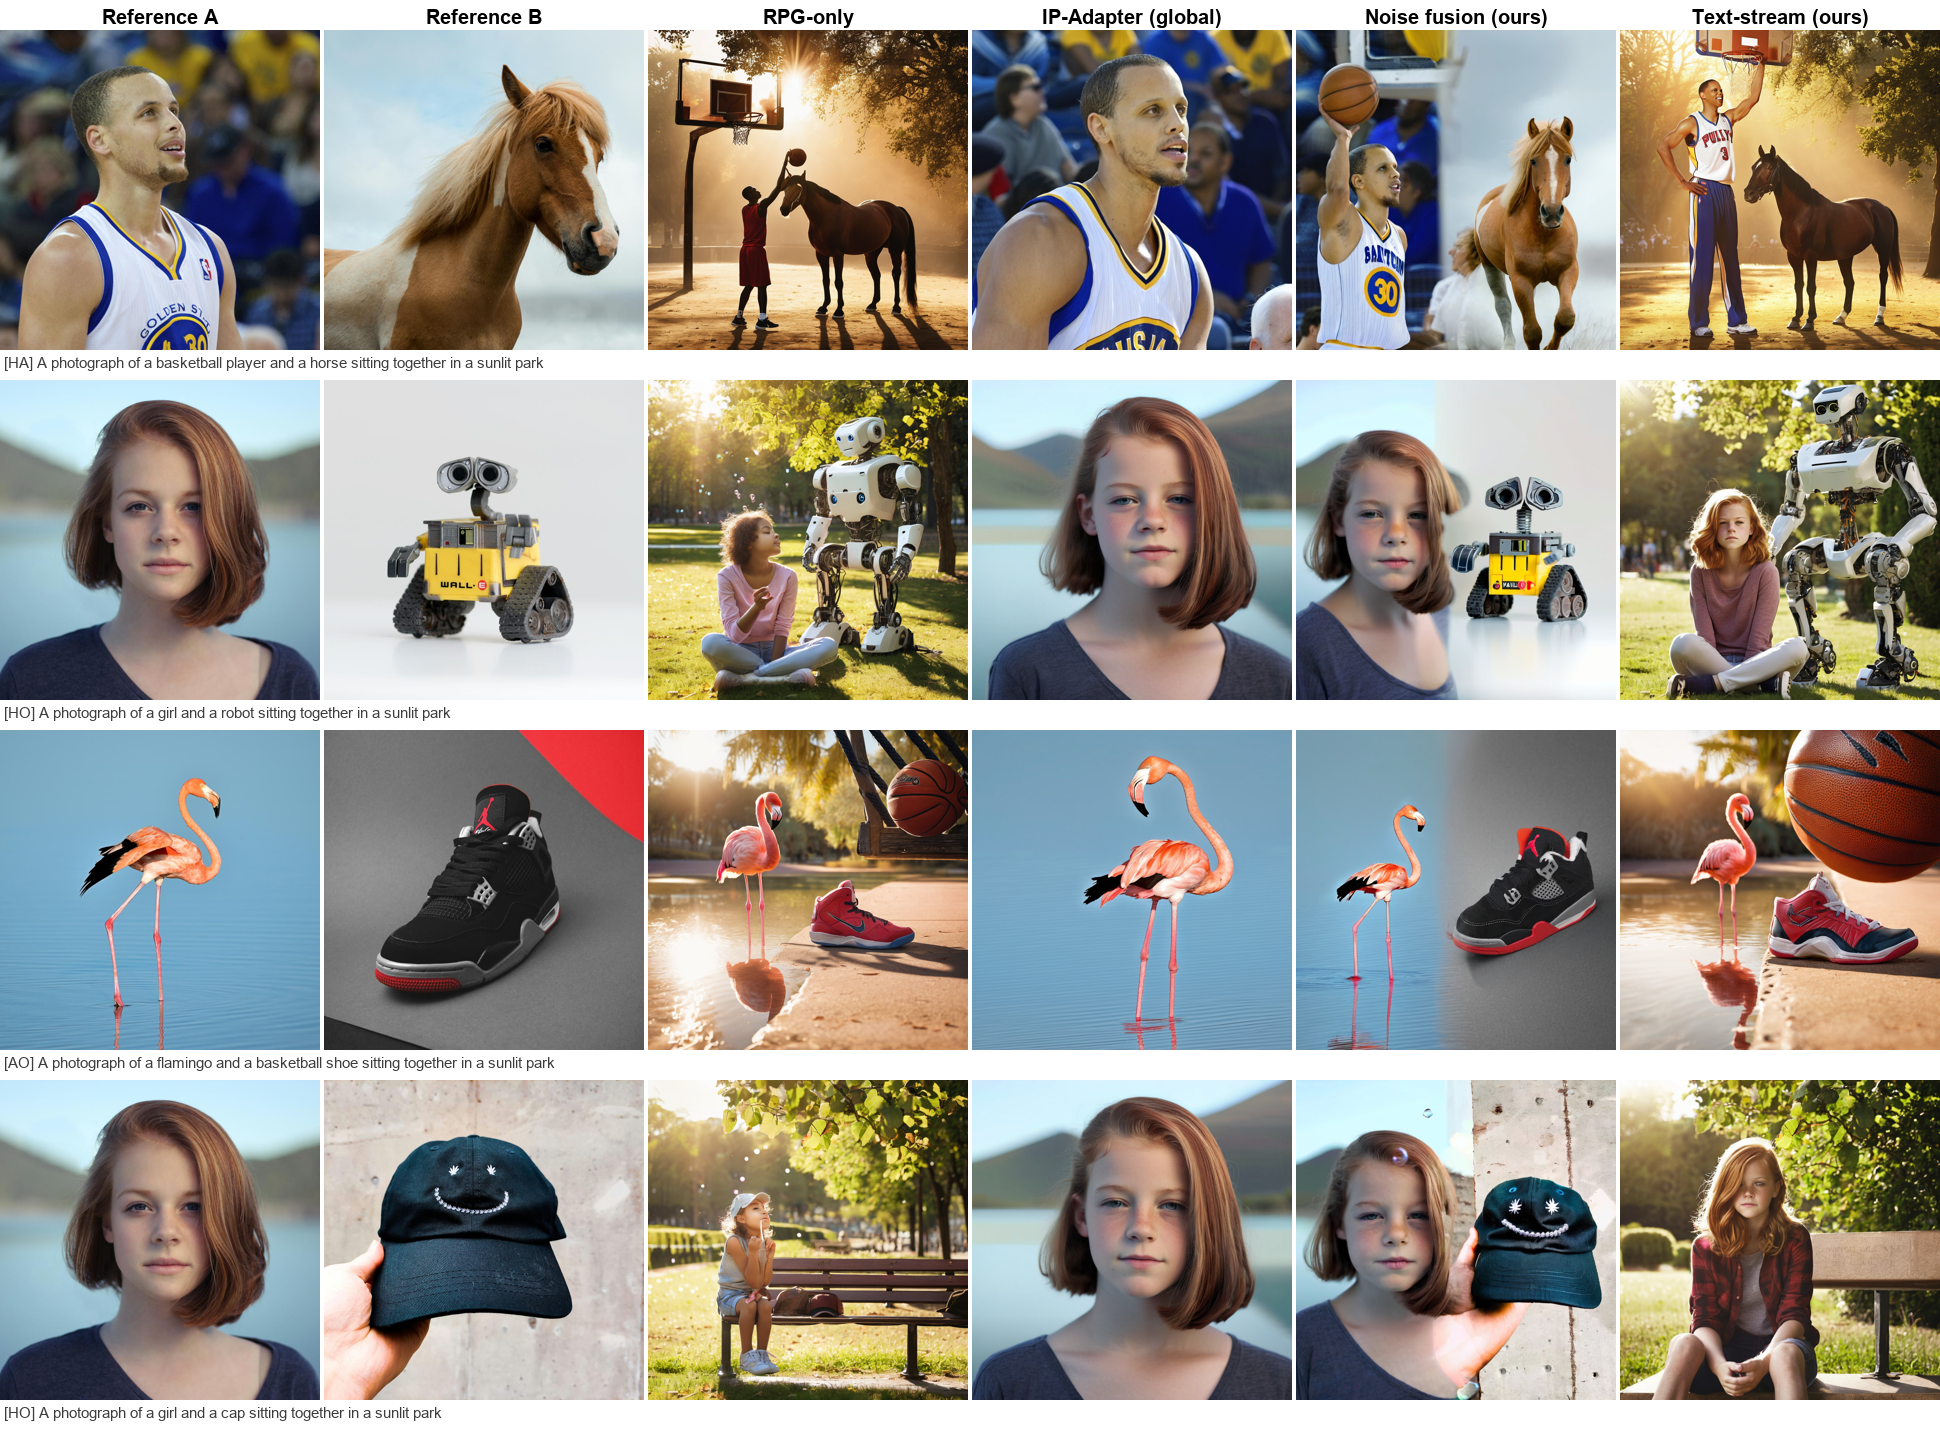
\includegraphics[width=\linewidth]{paper_figures/fig11_dreambench2_qual.png}
  \caption{%
    \textbf{Both operating points on four further DreamBench-2 pairs.}
    Same prompts, same seed, $1024$.  \emph{RPG-only} satisfies the prompt and
    ignores the references: the scene is a park, the subjects are generic.
    \emph{IP-Adapter (global)} reproduces the first reference and drops the
    second entirely.  The two rightmost columns are this paper's two operating
    points, and the trade between them is visible on every row.  \emph{Noise
    fusion} is the only configuration that reproduces the particular object---
    this robot rather than a robot, this shoe rather than a shoe---and it pays
    for that with the panel boundary the two regions meet at.  \emph{Text
    stream} composes one scene with a horse standing in it, a girl seated on
    the grass, a shoe on the ledge beside the water, and it loses the object's
    identity in doing so: the robot is no longer WALL-E and the cap is absent.
    Neither column is uniformly better, which is why we report both rather
    than designating one as the method.
  }
  \label{fig:db2_qual}
\end{figure*}

\noindent\textit{CLIP-T sits between the two baselines, and the reason is
worth stating plainly.}
Our CLIP-T ($0.623$) is below text-only RPG ($0.656$) and above global
IP-Adapter ($0.589$): conditioning on a reference pulls each region away from
the generic rendering a text prompt alone produces, and doing so regionally
costs less than doing it globally.  On this benchmark the effect is larger
than on Mixed-Eval-v1, and the cause is visible in the outputs.  DreamBench-2
references are photographs carrying their own scenes, our regions tile the
whole canvas so none of it is denoised as background, and a region therefore
tends to reproduce its reference's setting along with its subject---so a
prompt that relocates the subjects is only partly honoured.  This bounds how
the DINO-ID column should be read as well: similarity to a reference is
raised by reproducing its background, and the gain over the baselines is
larger here than on Mixed-Eval-v1 partly for that reason.  We return to it in
Section~\ref{sec:limitations}.

% ---- Section 4.4 ------------------------------------------------------------

\section{Qualitative Analysis}
\label{sec:qual}

% ---- Figure 3 ---------------------------------------------------------------
\begin{figure}[H]
  \centering
  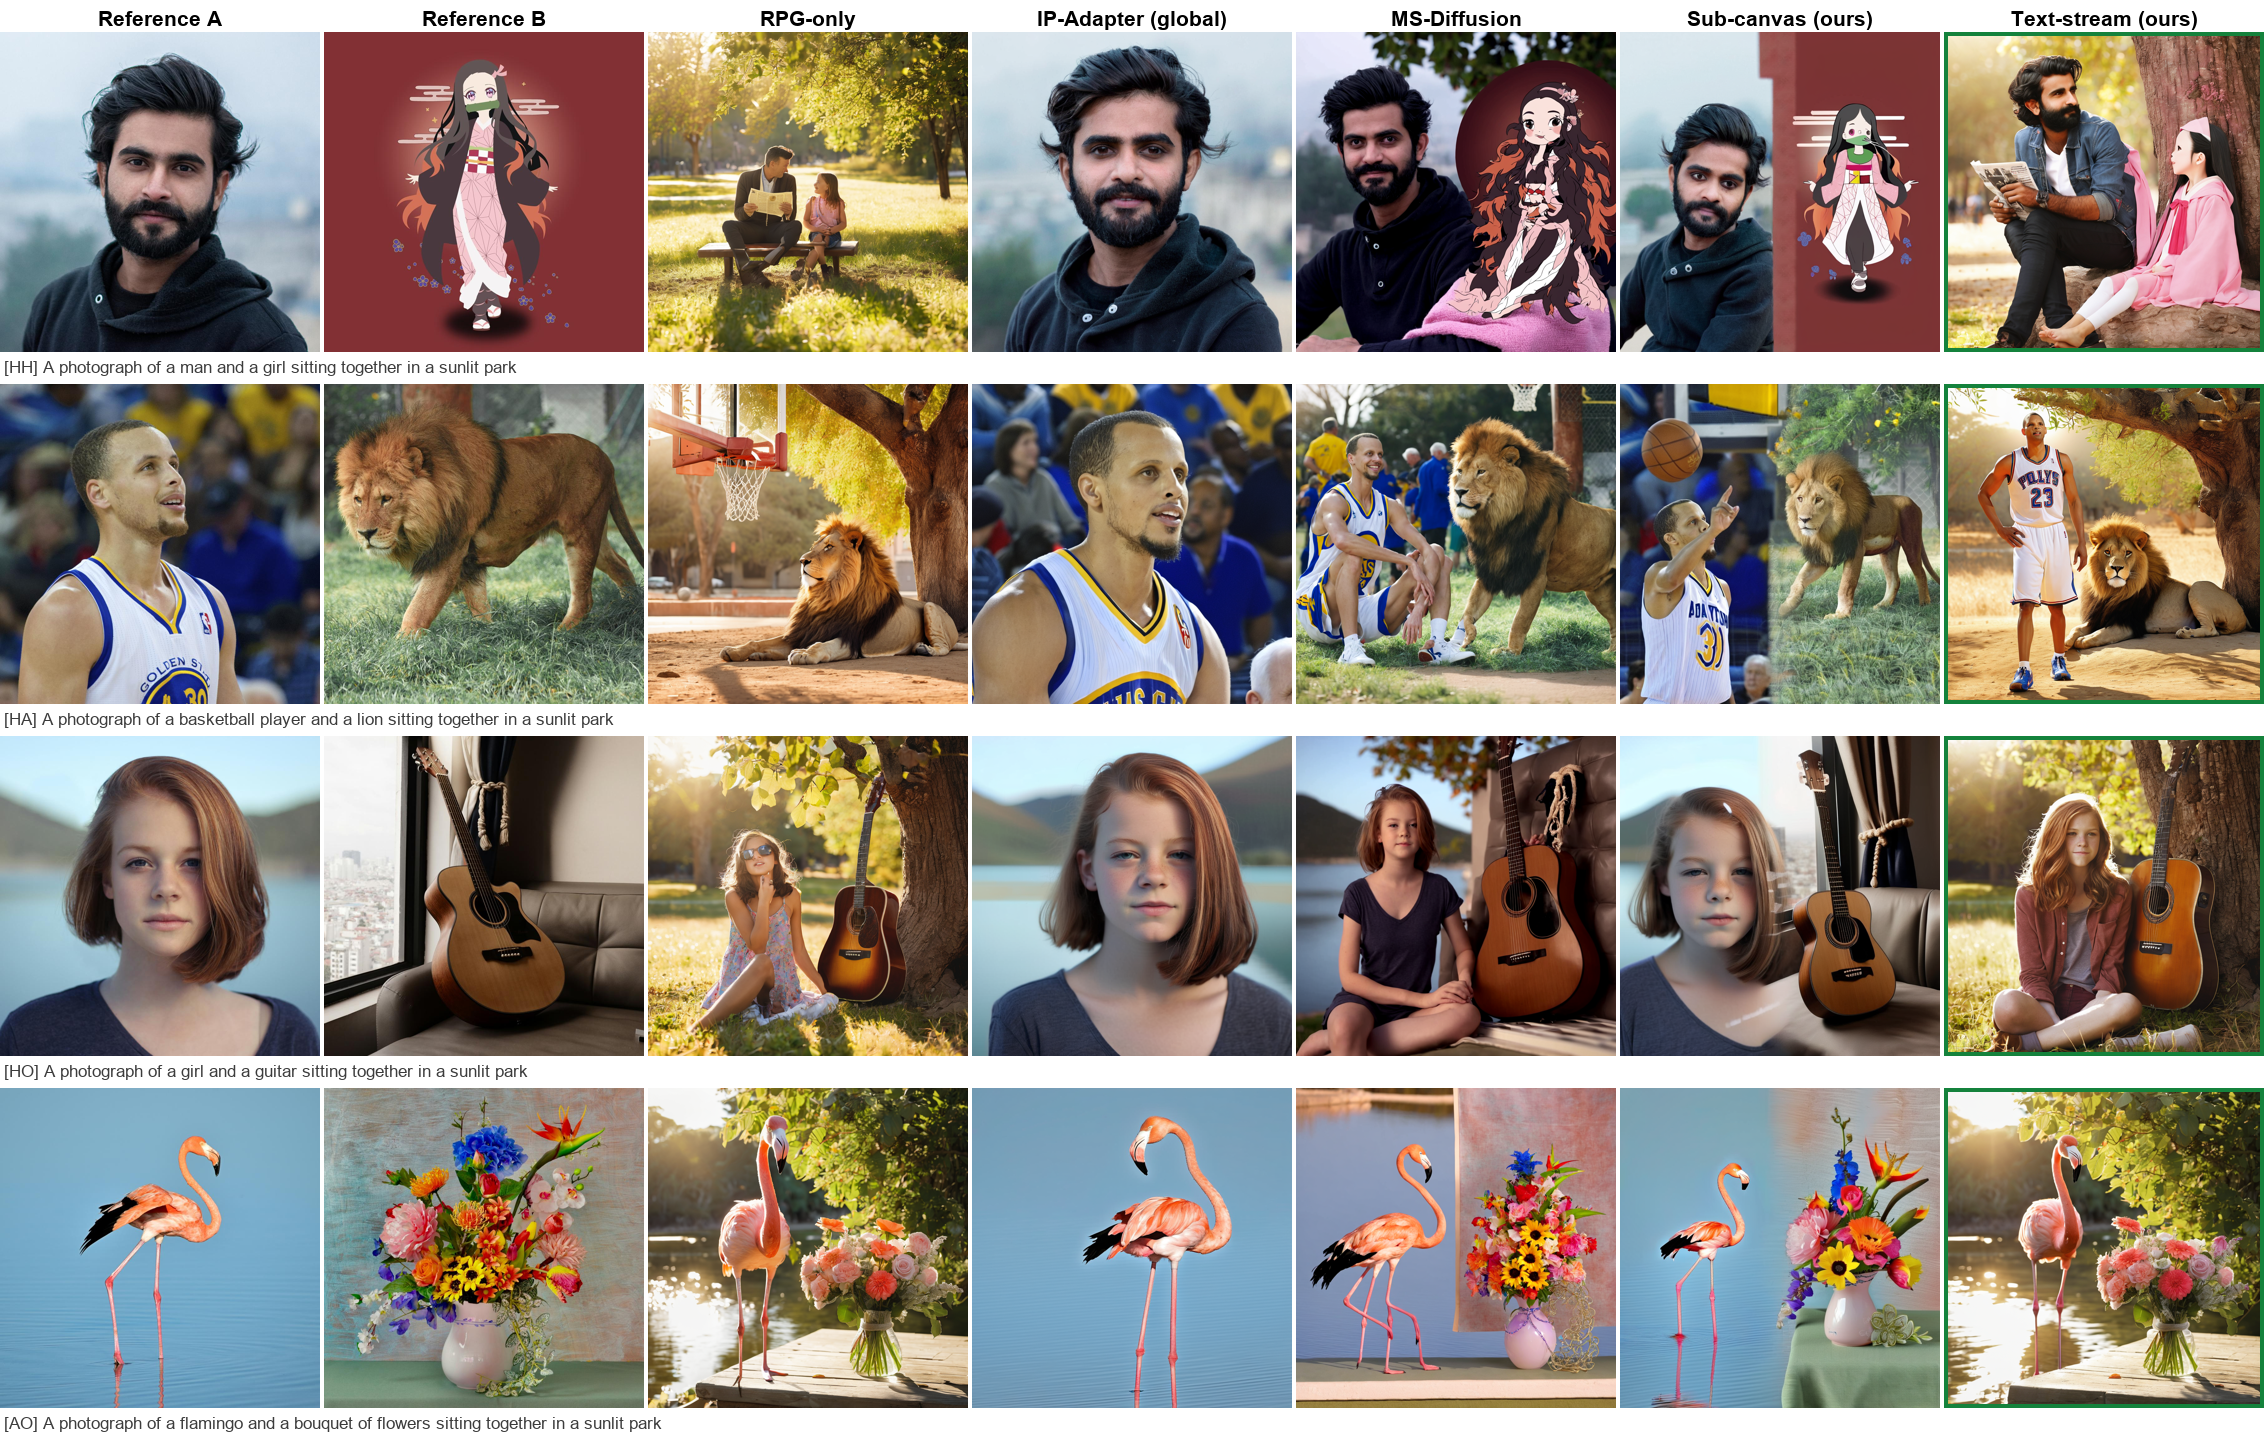
\includegraphics[width=\linewidth]{paper_figures/fig3_db2_qualitative.png}
  \caption{%
    \textbf{Qualitative comparison on DreamBench-2}, whose references are
    photographs of specific real subjects.  One sample per pair type, selected
    by a fixed rule---the lowest sample index within each type---rather than by
    inspection.  Sub-canvas compositing recovers both references but frames
    them as two panels meeting at the planner's boundary; the text-stream route
    puts them in the scene the prompt describes, at the cost of object identity
    (row~3's guitar and row~4's bouquet are generic, and row~4's fusion is
    skipped entirely because neither subject is a person).  Row~1 shows a
    further consequence of carrying identity as a face rather than as an image:
    the stylised reference is rendered as a photograph of a girl, since the
    fusion transfers facial identity and not the reference's illustration
    style.
  }
  \label{fig:qual}
\end{figure}

Fig.~\ref{fig:qual} shows three representative \emph{person}
comparisons; Fig.~\ref{fig:cross_cat} extends the comparison to
\emph{object} and \emph{mixed} categories.

\noindent\textit{Person samples.}
IP-Adapter (global) renders a single person, faithful to Reference~A, filling
the frame; the second identity is absent rather than merely contaminated.
Conceptrol produces one person too, but carrying traits of both references at
once.  Our sub-canvas compositing places two distinct people, each matching the
reference assigned to its region.

\noindent\textit{Object and mixed samples.}
Fig.~\ref{fig:cross_cat} shows the same pattern outside the face domain.
Given a watch and a chair, IP-Adapter~(global) returns the watch alone, and
Conceptrol returns a single hybrid object that fuses the two.  Our method
places both objects, each in its planned region, across all category types.

\begin{figure}[H]
  \centering
  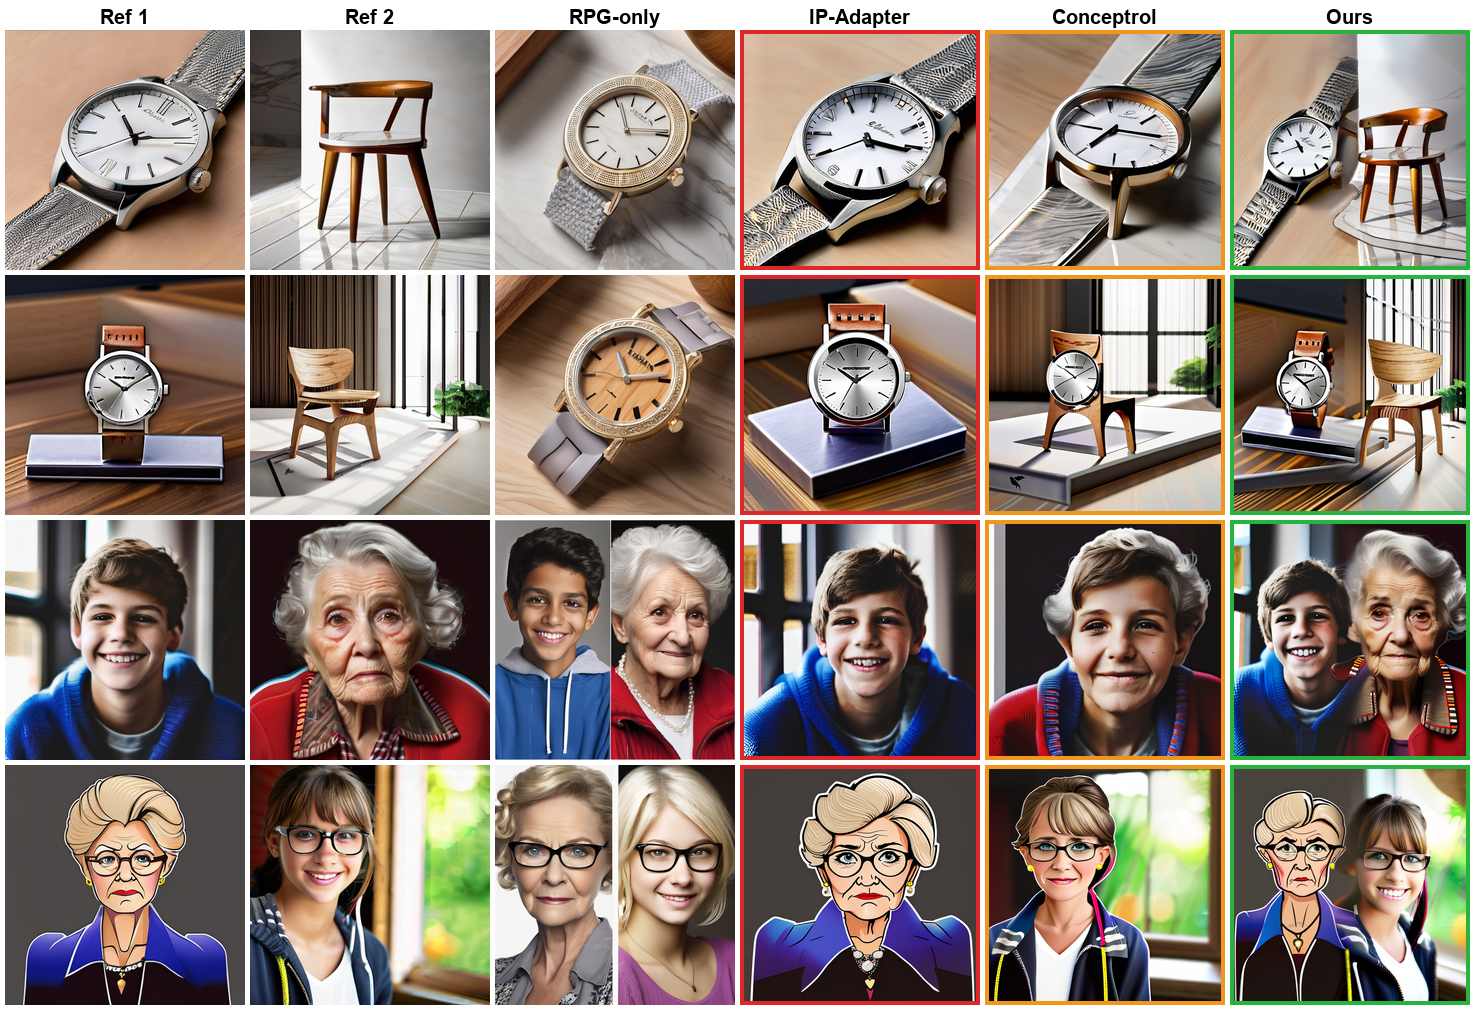
\includegraphics[width=\linewidth]{paper_figures/fig5_cross_category.png}
  \caption{%
    \textbf{Cross-category generalisation.}
    Top two rows: object samples.  Bottom two rows: mixed-scene samples.
    IP-Adapter (global, red border) leaks one object's texture or
    colour into the other region.  Our method (green border) correctly
    assigns each reference to its own region across all category types.
  }
  \label{fig:cross_cat}
\end{figure}

% ---- Table 2 ----------------------------------------------------------------

\section{Ablation Study}

\begin{table}[htbp]
\centering
\caption{%
  \textbf{Where the spatial constraint is applied.}
  All rows use the same MLLM plan, the same references and the same
  adapter weights; they differ in \emph{where} the regions are separated
  and, for the two attention-gated rows, in how strongly the injection is
  attenuated.  \emph{Attenuated} stacks the per-layer, per-timestep and
  per-category gates that a leakage-suppressing configuration typically
  applies; \emph{full strength} removes all of them and runs at the same
  $\lambda{=}0.8$ as our method.  Neither exceeds the text-only baseline
  on any identity axis.  Moving the constraint into the sampling loop
  does, and denoising per-region sub-canvases rather than the full canvas
  is what additionally fixes the chimeric-subject failure.  Binding accuracy
(Section~\ref{sec:binding}) separates the same rows independently of
identity: $0.632$ for attention gating against $0.610$ for the text-only
baseline, and $0.938$ for ours.
  All rows use $\tau{=}1$ (late release off) so that this table isolates
  the fusion geometry; the default $\tau{=}0.7$ used elsewhere is
  evaluated separately in Table~\ref{tab:tau}.%
}
\label{tab:ablation}
\resizebox{\columnwidth}{!}{%
\begin{tabular}{lccccc}
\toprule
Separation mechanism & DINO-ID & Margin & CLIP-T & ArcFace & Spec. \\
\midrule
None (text only, RPG)          & 0.352 & $+$0.076 & 0.650 & 0.129 & 0.082 \\
None (global adapter)          & 0.341 & $-$0.082 & 0.615 & 0.089 & 0.076 \\
\midrule
Attention, box mask            & 0.358 & $+$0.098 & \textbf{0.652} & 0.122 & 0.089 \\
Attention, semantic mask       & 0.387 & $+$0.004 & 0.630 & 0.165 & 0.090 \\
Attention, box $\cap$ semantic & 0.593 & $+$0.353 & 0.651 & 0.243 & 0.189 \\
\midrule
Noise fusion, full-canvas    & 0.603 & $+$0.398 & 0.641 & 0.212 & 0.185 \\
\textbf{Noise fusion, sub-canvas (Ours)}
                             & \textbf{0.719} & \textbf{$+$0.490}
                             & 0.646 & \textbf{0.264} & \textbf{0.249} \\
\bottomrule
\end{tabular}
}
\end{table}

\noindent\textit{The cascade a reader would propose, run to its end.}
The rungs above gate the adapter inside a pipeline driven by a single global
prompt.  The obvious objection is that we never combined the two halves that
matter: RPG's regional \emph{text} attention, which is what makes its
compositions read as photographs, and Conceptrol's semantic mask, which is
what keeps a reference's texture off the background.  Cascade them---the
planner supplies $M_{\mathrm{spatial}}$, the region's own text attention
supplies $M_{\mathrm{semantic}}$, and the adapter writes only where both
agree---and the identity should arrive without the leakage.

We implemented that cascade inside RPG.  The semantic map costs nothing extra
there: RPG's regional attention already computes the queries and keys the map
is read from, so no hook and no second forward pass are needed.  We then ran
it at full injection strength on 24 photographic human-human pairs, framed as
medium shots so that faces occupy about $9.5\%$ of the canvas and identity has
room to be visible.

\begin{table}[htbp]
\centering
\caption{%
  \textbf{The RPG cascade delivers RPG's pictures and none of the identity.}
  ArcFace on detected faces, so the score does not move with framing; $0$ is
  chance.  Text-only RPG is the floor.  Adding the adapter, with or without the
  semantic mask, and at five times the default strength, never leaves it.%
}
\label{tab:cascade}
\resizebox{\columnwidth}{!}{%
\begin{tabular}{lccc}
\toprule
Configuration & ArcFace & Faces/img & Face area \\
\midrule
RPG, text only                       & $+$0.014 & 1.96 & \phantom{0}9.48\% \\
\midrule
$+$ IP-Adapter, box mask             & $+$0.003 & 1.88 & \phantom{0}4.97\% \\
$+$ IP-Adapter, box $\cap$ semantic  & $-$0.010 & 1.79 & \phantom{0}7.31\% \\
\quad the same, binarised mask       & $+$0.004 & 1.88 & \phantom{0}5.21\% \\
\midrule
box $\cap$ semantic, $\lambda{=}1.5$ & $+$0.014 & 1.88 & \phantom{0}6.20\% \\
box $\cap$ semantic, $\lambda{=}3.0$ & $-$0.008 & 1.75 & \phantom{0}4.54\% \\
\bottomrule
\end{tabular}%
}
\end{table}

Table~\ref{tab:cascade} is the answer, and it is flat.  The pictures are
RPG's---medium framing, natural poses, no boundary---and the people in them
are not the reference people.  Raising $\lambda$ from $0.6$ to $3.0$ does not
change that; it only degrades the image, blurring faces and oversaturating
colour while the face count falls.  The semantic mask cannot help, because a
mask restricts where identity is written and there is no identity to restrict:
the box-gated row is already at chance.

This closes the question the ladder opens.  Attention-level gating recovers
$1.7\%$ of the identity the same adapter delivers from the sampling loop when
measured in the Conceptrol pipeline; measured inside RPG, with the strongest
mask the two systems can jointly produce and five times the injection
strength, it recovers none.  The sub-canvas construction is not a preference
over a simpler cascade.  The simpler cascade does not work.

\noindent\textit{The site of the constraint, not its presence,
determines identity.}
The two attention-gated rows bracket the injection strength available to
that formulation---one heavily attenuated, one with every gate removed
and $\lambda$ raised to our own setting---and neither approaches the rest
of the table.  The attenuated variant reproduces the text-only baseline
literally, on 41 of 150 images bit-for-bit.  The full-strength variant
reproduces none of them and does clear the baseline on DINO-ID and Margin,
by $+0.018$ and $+0.022$ respectively, but leaves ArcFace and specificity
(Section~\ref{sec:specificity}) untouched and closes only about a
twentieth of the distance to noise-level fusion.  Injection strength is
therefore not what separates these rows from the rest of the table.  Relocating the identical adapter to
noise-level fusion lifts DINO-ID to $0.561$ and Margin to $+0.350$
without any change to the adapter or its scale---the gain comes from
\emph{where} the spatial constraint is imposed.

We note that recent training-free multi-concept methods
\cite{he2025conceptrol,mc2_2025,latexblend2025,freecustom2024,yu2025anyms}
differ in how they compute or refine the attention mask but all inject
and confine identity \emph{within} the attention operator, i.e.\ they
instantiate Eq.~\ref{eq:gated}.  Our attention-gated rows are one
implementation of that formulation, not a reimplementation of any of
these methods, and we do not claim to have measured them: a different
masking heuristic could plausibly behave differently.  What our
measurement does establish is that the shortfall is not explained by
weak injection, since removing every attenuation does not move any
identity axis.

\noindent\textit{Sub-canvas vs.\ full-canvas.}
Full-canvas fusion already recovers most of the identity, but each
per-concept pass composes its subject at the centre of the frame, so
for centred subjects the masks splice two half-subjects into one.
Confining each pass to its own sub-canvas raises DINO-ID further
($0.561\!\to\!0.647$) and Margin ($+0.350\!\to\!+0.415$), and---more
importantly---removes the chimeric-subject artefact that the metrics
only partly capture (Fig.~\ref{fig:ablation_vis}).  ArcFace is
unchanged ($0.268$ vs.\ $0.269$) because it is measured on the
face crop, which is intact in both; the difference is whether that face
belongs to one coherent person or is stitched from two.

\begin{figure}[H]
  \centering
  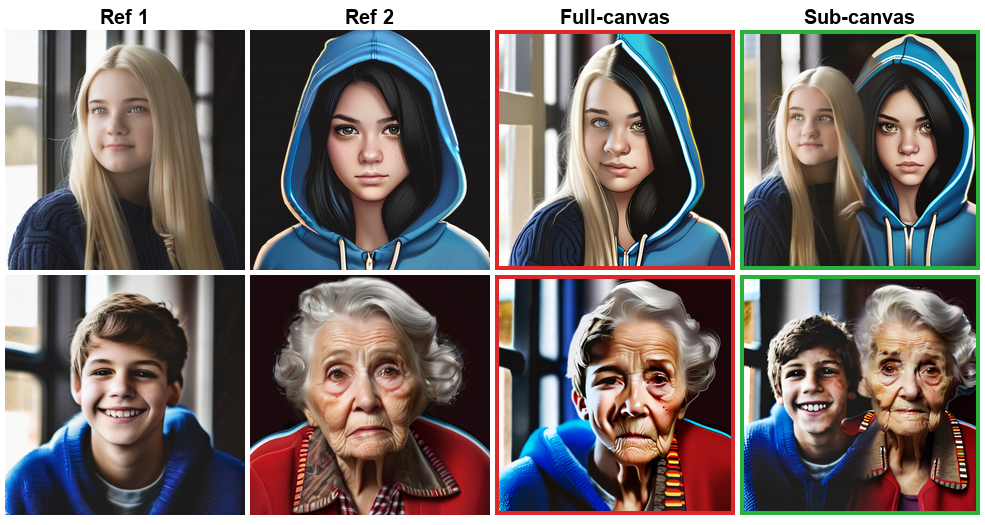
\includegraphics[width=\linewidth]{paper_figures/fig6_ablation_visual.png}
  \caption{%
    \textbf{Full-canvas vs.\ sub-canvas fusion.}
    Same inputs, same full-strength adapter, same fusion weights.
    \emph{Full-canvas}: each concept is denoised over the whole frame,
    so both subjects form at the centre and the masks merge them into a
    single chimeric face.
    \emph{Sub-canvas}: each concept is denoised inside its own
    region, so the two subjects are distinct and correctly placed.
    Both columns use $\tau{=}1$ to isolate the fusion geometry from the
    late release of Section~\ref{sec:tau}.
  }
  \label{fig:ablation_vis}
\end{figure}

% ---- tau sweep --------------------------------------------------------------

\section{Where the Release Point Comes From}
\label{sec:commitment}

Table~\ref{tab:tau} is an observational sweep, and a flat curve admits two
readings.  Identity may be settled before the release, so the late steps
\emph{cannot} move it; or the late steps may retain the ability to move it and
merely not exercise it on this benchmark.  The design of
Section~\ref{sec:late_release} assumes the first, as does the wider
literature---Personalize Anything~\cite{feng2026personalize} injects
aggressively early and regularises late on that premise, and acceleration work
reports identity stabilising within the first handful of
steps~\cite{zheng2026fewsteps}---but a sweep cannot distinguish the two.  An
intervention can.

\noindent\textit{Protocol.}
We denoise each of the 30 reference-swap samples of
Section~\ref{sec:refresponse} with region~0 carrying its own reference $A$ for
the first $k$ steps and the same-category alternative $A'$ for the remaining
$30-k$.  The regional decomposition runs for the whole trajectory
($\tau{=}1$), so the reference is the only thing that changes at step $k$;
prompt, layout, seed and region~1's reference are untouched.  On region~0's
crop we report
\begin{align}
  A(k) &= \operatorname{sim}(\mathrm{crop}_0,A')
        - \operatorname{sim}(\mathrm{crop}_0,A), \label{eq:swapA}\\
  F(k) &= D(k)\,/\,D(0), \label{eq:swapF}
\end{align}
with $D$ as in Eq.~\ref{eq:swapD}, measured against the never-swapped render.
$A(k)$ asks which reference the output ended up resembling and needs no
anchor; its zero crossing is the commitment point.  $F(k)$ is the fraction of
the achievable identity change that a swap at step $k$ can still buy.  We also
report $S(k)$, the pixel distance from the never-swapped render, to separate
\emph{the trajectory stopped responding} from \emph{the trajectory still
responds but no longer with identity}.

$k{=}0$ and $k{=}30$ are boundary controls rather than measurements.  A
further control is available because $k{=}30$ is, by construction, an ordinary
$\tau{=}1$ render: it reproduces the independently generated $\tau{=}1$ image
of the same sample to a mean absolute difference of $0.03$ of $255$, so the
probe samples the trajectory this paper reports and not a re-implementation of
it.

\begin{table}[htbp]
\centering
\caption{%
  \textbf{Identity commitment.}  Region~0's reference is replaced by a
  same-category instance at step $k$ of $30$, with the regional decomposition
  active throughout and everything else fixed (30 samples).
  $S$: pixel distance from the never-swapped render.
  $A$ (Eq.~\ref{eq:swapA}): positive when the output resembles the newly
  supplied reference, negative when the first $k$ steps had already decided.
  $F$ (Eq.~\ref{eq:swapF}): fraction of the achievable identity change still
  available at step $k$.  $p$ is a two-sided paired $t$ test on $A$.
  The choice of subject stops being reversible at $k{\approx}6$, a fifth of
  the way through the trajectory.%
}
\label{tab:commitment}
\resizebox{\columnwidth}{!}{%
\begin{tabular}{cccccc}
\toprule
$k$ & $k/30$ & $S$ & $A$ & $p$ & $F$ \\
\midrule
0  & 0.00 & 55.75 & $+0.481$ & $<0.001$ & 1.000 \\
2  & 0.07 & 49.77 & $+0.405$ & $<0.001$ & 0.916 \\
4  & 0.13 & 41.71 & $+0.258$ & $<0.001$ & 0.751 \\
6  & 0.20 & 32.46 & $+0.034$ & 0.61     & 0.538 \\
9  & 0.30 & 21.27 & $-0.222$ & $<0.001$ & 0.323 \\
12 & 0.40 & 11.96 & $-0.368$ & $<0.001$ & 0.188 \\
15 & 0.50 &  6.11 & $-0.456$ & $<0.001$ & 0.128 \\
30 & 1.00 &  0.00 & $-0.590$ & $<0.001$ & 0.000 \\
\bottomrule
\end{tabular}%
}
\end{table}

\noindent\textit{The choice of subject is made in the first fifth of the
trajectory.}
$A(k)$ crosses zero at $k{=}6.2$ and $F(k)$ falls through a half at $k{=}5.9$:
two estimators, one anchored and one not, agree on $\tau^{*}{\approx}0.21$.
Before step 6 the incoming reference still wins; after it, the output
resembles the reference the first six steps saw, however many steps the new
one is given.  By $k{=}15$---half the trajectory, and well past our default
release point---a swap buys only
$13\%$ of the achievable change and the output still sits $0.397$ closer to
the original reference than to the one actually driving 24 of the 30 steps.
One caveat bounds this: the sub-prompt is written for $A$ and is not swapped,
so $A$ carries a standing text advantage and the crossing is a lower bound on
where the reference alone could still reverse the choice.

\noindent\textit{The trajectory keeps responding after it stops carrying
identity.}
At $k{=}6$ the swap still moves the image by $S{=}34.7$ of $255$---three
fifths of a full-trajectory swap---while $A$ is indistinguishable from zero.
This is the dissociation of Section~\ref{sec:refresponse} in time rather than
across methods: late injection perturbs the image without changing whose
identity it carries.  A study that measured only how much the output moved
would place the commitment point far later than it is.

\noindent\textit{The release point is not set by identity.}
If identity commitment were the constraint, $\tau{=}0.21$ would suffice.  It
does not: at $\tau{=}0.3$ binding accuracy is $0.828$ against $0.928$ at
$\tau{=}1$, still a tenth short, and it does not saturate until
$\tau{\approx}0.7$ (Table~\ref{tab:tau}).  What the regional phase buys
between $\tau^{*}$ and our default is therefore not the choice of subject,
which was settled at $0.21$, but the isolation of the subjects from each
other.  The trade-off the switch point actually governs is isolation against
whatever the released phase provides---the same conclusion
Section~\ref{sec:binding} reached from the opposite direction, that the
release costs placement rather than identity---and we set $\tau$ at $0.7$,
where isolation is still at its maximum and the identity settled at $0.21$ is
not disturbed.

% ---- Table 3 ---------------------------------------------------------------


\section{Per-Category Analysis}

\begin{table}[htbp]
\centering
\caption{%
  \textbf{Per-category ArcFace identity} on Mixed-Eval-v1
  (Ours at the default $\tau{=}0.7$).
  Person: portrait samples; Mixed: scene samples with faces.
  Detect rate shows fraction of regions where ArcFace detected a face.
}
\label{tab:percategory}
\resizebox{\columnwidth}{!}{%
\begin{tabular}{lccccc}
\toprule
Method & \multicolumn{2}{c}{Person} & \multicolumn{2}{c}{Mixed} & Overall \\
\cmidrule(lr){2-3}\cmidrule(lr){4-5}
       & ArcFace$\uparrow$ & Det.Rate & ArcFace$\uparrow$ & Det.Rate & ArcFace$\uparrow$ \\
\midrule
RPG-only           & 0.130 & 0.76 & 0.133 & 0.56 & 0.131 \\
IP-Adapter (global)& 0.103 & 0.55 & 0.093 & 0.55 & 0.101 \\
\textbf{Ours}      & \textbf{0.265} & 0.88 & \textbf{0.282} & 0.58 & \textbf{0.272} \\
\bottomrule
\end{tabular}%
}
\end{table}

\noindent\textit{Identity gains are strongest where faces are present.}
Table~\ref{tab:percategory} breaks ArcFace down by category.  The
detection rate is as informative as the score here.  Global IP injection
reaches ArcFace $0.103$ on person samples---close to text-only ($0.130$)---but
its detection rate collapses from $0.76$ to $0.55$, because the frame that
should hold two faces holds one; the score is computed on whichever single face
survives.  Sub-canvas compositing instead lifts ArcFace by roughly $80\%$ on
person ($0.130\!\to\!0.235$) and mixed ($0.133\!\to\!0.271$) splits \emph{and}
raises the person detection rate to $0.88$---the generated faces are more
numerous, better formed, and closer to the reference identity at the same time.

\section{Scaling to More Regions}
\label{sec:scaling}

\begin{figure}[H]
  \centering
  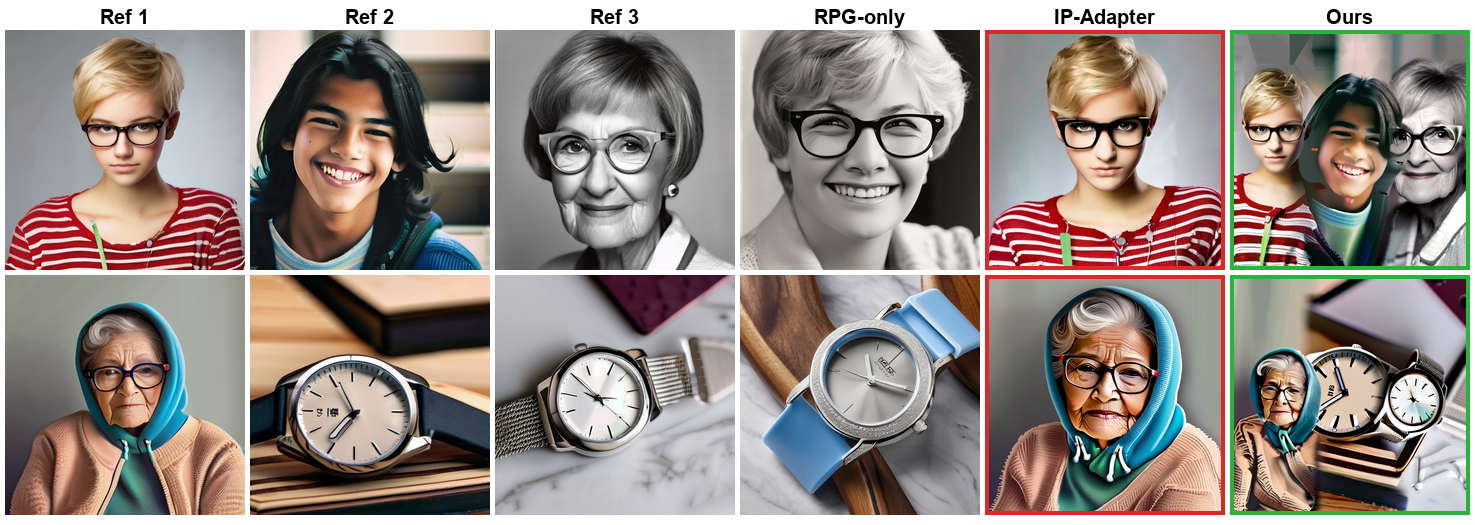
\includegraphics[width=\linewidth]{paper_figures/fig7_three_region.png}
  \caption{%
    \textbf{Three-region generalisation ($N{=}3$).}
    The construction extends to three simultaneous reference concepts
    without modification.  IP-Adapter (global) is conditioned on one
    reference and renders it alone, so the other two concepts are absent.
    Sub-canvas compositing places all three, and the quantitative form of
    that observation is the $N{=}3$ column of Table~\ref{tab:binding}
    ($0.898$ against $0.800$, $p{=}0.0001$).
    The second row also shows the failure the geometry does not prevent:
    with one person and two similar objects the person is composed inside a
    region narrower than a portrait wants, and is rendered at a scale that
    does not match the objects beside it.  Region width is fixed by the
    planner's split ratio and is not adapted to what each region contains
    (Section~\ref{sec:limitations}).
  }
  \label{fig:three_region}
\end{figure}

The construction imposes no upper bound on $N$: the MLLM planner assigns one
reference per region, and the $N$ sub-canvases $\{\Omega_i\}$ partition the
latent, each denoised by its own single-concept adapter pass and fused by
Eq.~\ref{eq:fuse}.  Fig.~\ref{fig:three_region} shows $N{=}3$ person
samples from Mixed-Eval-v1: the per-region isolation holds, whereas global
injection produces an indistinct blend across all three regions.

Whether it keeps holding is a measurement rather than a corollary, and the
structural argument runs in our favour: a sub-canvas is denoised in its own
window, so a region's problem does not depend on how many other regions
exist, whereas a trained layout-conditioned model has no such guarantee.  We
tested it.  \emph{Scaling-Bench} extends the same task to $N\in\{4,5,6\}$
with 30 samples per region count (90 total, 10 per category per count),
scored with the region-level binding accuracy of Section~\ref{sec:binding}.
That metric is the one instrument here that stays interpretable as $N$ grows,
since it is internal to a single image and its chance level $1/N$ is known
exactly.

\begin{table}[htbp]
\centering
\caption{%
  \textbf{Region-level binding accuracy against region count.}
  Scaling-Bench, 30 samples per $N$; the $N{=}2,3$ columns are the
  Mixed-Eval-v1 numbers of Table~\ref{tab:binding}, repeated for continuity.
  $\Delta$ and $p$ compare our default ($\tau{=}0.7$) against MS-Diffusion,
  paired and two-sided; the $\tau{=}0.5$ row is kept to separate the release
  point's contribution from the method's.  Both methods stay above chance at
  every $N$, and the gap between them grows monotonically with the number of
  regions, from $+0.006$ at two to $+0.194$ at six.%
}
\label{tab:scaling}
\resizebox{\columnwidth}{!}{%
\begin{tabular}{lccccc}
\toprule
$N$ & 2 & 3 & 4 & 5 & 6 \\
\midrule
chance               & 0.500 & 0.333 & 0.250 & 0.200 & 0.167 \\
MS-Diffusion         & 0.967 & 0.871 & 0.725 & 0.600 & 0.439 \\
Ours ($\tau{=}0.5$)  & --- & --- & 0.808 & 0.700 & 0.539 \\
\textbf{Ours} ($\tau{=}0.7$) & \textbf{0.973} & \textbf{0.902} & \textbf{0.825}
                     & \textbf{0.713} & \textbf{0.633} \\
\midrule
$\Delta$ ($\tau{=}0.7$) & $+$0.006 & $+$0.031 & $+$0.100 & $+$0.113
                     & $+$0.194 \\
$p$                  & 0.66 & 0.18 & 0.060 & 0.020 & $<$0.001 \\
\bottomrule
\end{tabular}%
}
\end{table}

The structural argument survives, and it is the clearest result in the
paper's favour.  The two methods do not degrade at the same rate: least
squares over $N{=}2\ldots6$ gives $-0.133$ accuracy per added region for
MS-Diffusion against $-0.087$ for ours, a third slower.  The gap grows
monotonically---$+0.006$, $+0.031$, $+0.100$, $+0.113$, $+0.194$---and
becomes significant where it matters most, at $N{=}5$ ($p{=}0.020$) and
$N{=}6$ ($p{<}0.001$), the region counts at which a trained
layout-conditioned model is closest to chance.  At six regions MS-Diffusion
retains $+0.272$ above chance and we retain $+0.466$.

This is what the sub-canvas construction was supposed to buy and, at $768$,
did not.  We report the earlier result because the reason for the difference
is instructive.  A sub-canvas is denoised at the size of its own region, so
at $N{=}6$ on a $768$ canvas each pass runs on a $128$-pixel-wide strip, far
outside the range SDXL was trained on; at $1024$ the same strip is $171$
pixels.  What limits the construction at high $N$ is therefore not the
per-region independence but the resolution that independence leaves each
region, and a backbone evaluated below its native size hides exactly the
advantage the construction is meant to have.  A trained model that reasons
over the whole canvas has no such floor, which is why it loses less from the
smaller canvas and gains less from the larger one.

\begin{figure}[htbp]
  \centering
  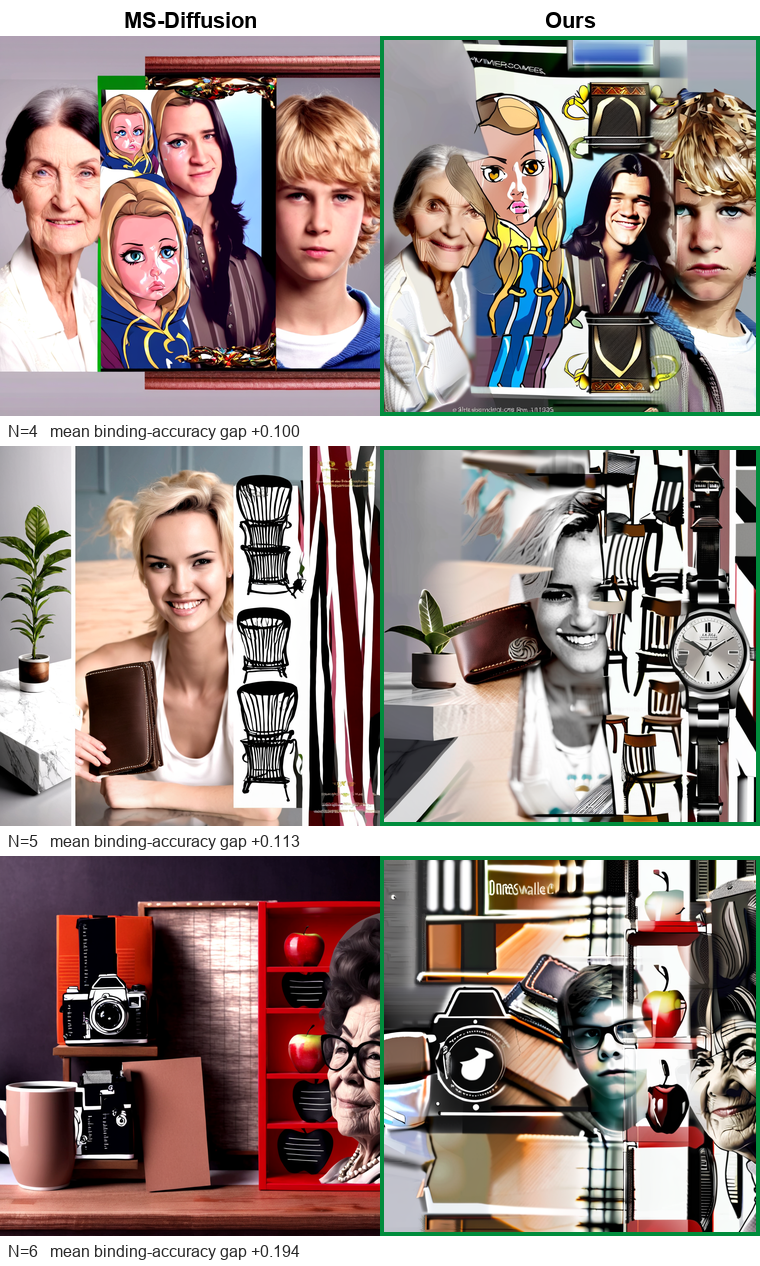
\includegraphics[width=\linewidth]{paper_figures/fig12_scaling.png}
  \caption{%
    \textbf{What the scaling advantage does and does not look like.}
    One sample per region count, chosen by a fixed rule: within each count we
    show the sample whose binding-accuracy gap is closest to the mean gap for
    that count, so the row is typical of the measured difference rather than
    its best case.
    The measured advantage is real---our regions hold the concepts they were
    assigned more often---but the figure shows what the number does not: at
    $N\!\ge\!4$ neither method produces an image a user would keep.  Ours
    fragments into strips with visible stylistic discontinuities; MS-Diffusion
    stays more photographic while binding fewer regions correctly.  Part of
    the disorder is the benchmark's, since Scaling-Bench draws its references
    from the Mixed-Eval-v1 pool whose styles are uncontrolled
    (Section~\ref{sec:exp}), and part is the method's.  We report the figure
    beside the table because the table alone would overstate the result.%
  }
  \label{fig:scaling_visual}
\end{figure}

\noindent\textit{The advantage is in placement, not in usable images.}
Fig.~\ref{fig:scaling_visual} puts the three region counts beside each
other, and it qualifies the result above in a way the table cannot.  At
$N\!\ge\!4$ neither method produces an image that would survive any practical
use: ours breaks into strips with visible stylistic seams, MS-Diffusion holds
a more photographic composition while placing fewer concepts where they
belong.  What Scaling-Bench establishes is therefore that the sub-canvas
construction keeps assigning concepts to their regions further into a regime
where both methods have already stopped producing usable output---a statement
about the mechanism's degradation, not a claim that the method is useful at
six regions.  The practical range of the method, on this evidence, is the
$N\!\le\!3$ of Mixed-Eval-v1.

\noindent\textit{The release point contributes little of this.}
Holding resolution fixed, moving $\tau$ from $0.5$ to $0.7$ is worth
$+0.017$ at $N{=}4$ ($p{=}0.48$), $+0.013$ at $N{=}5$ ($p{=}0.70$) and
$+0.094$ at $N{=}6$ ($p{=}0.001$).  Only the last is significant and we
report it uncorrected for three tests, so the honest reading is that the
release point costs little at any region count rather than that it helps at
high ones.  The separation above is the geometry's, not the schedule's.

\begin{figure}[H]
  \centering
  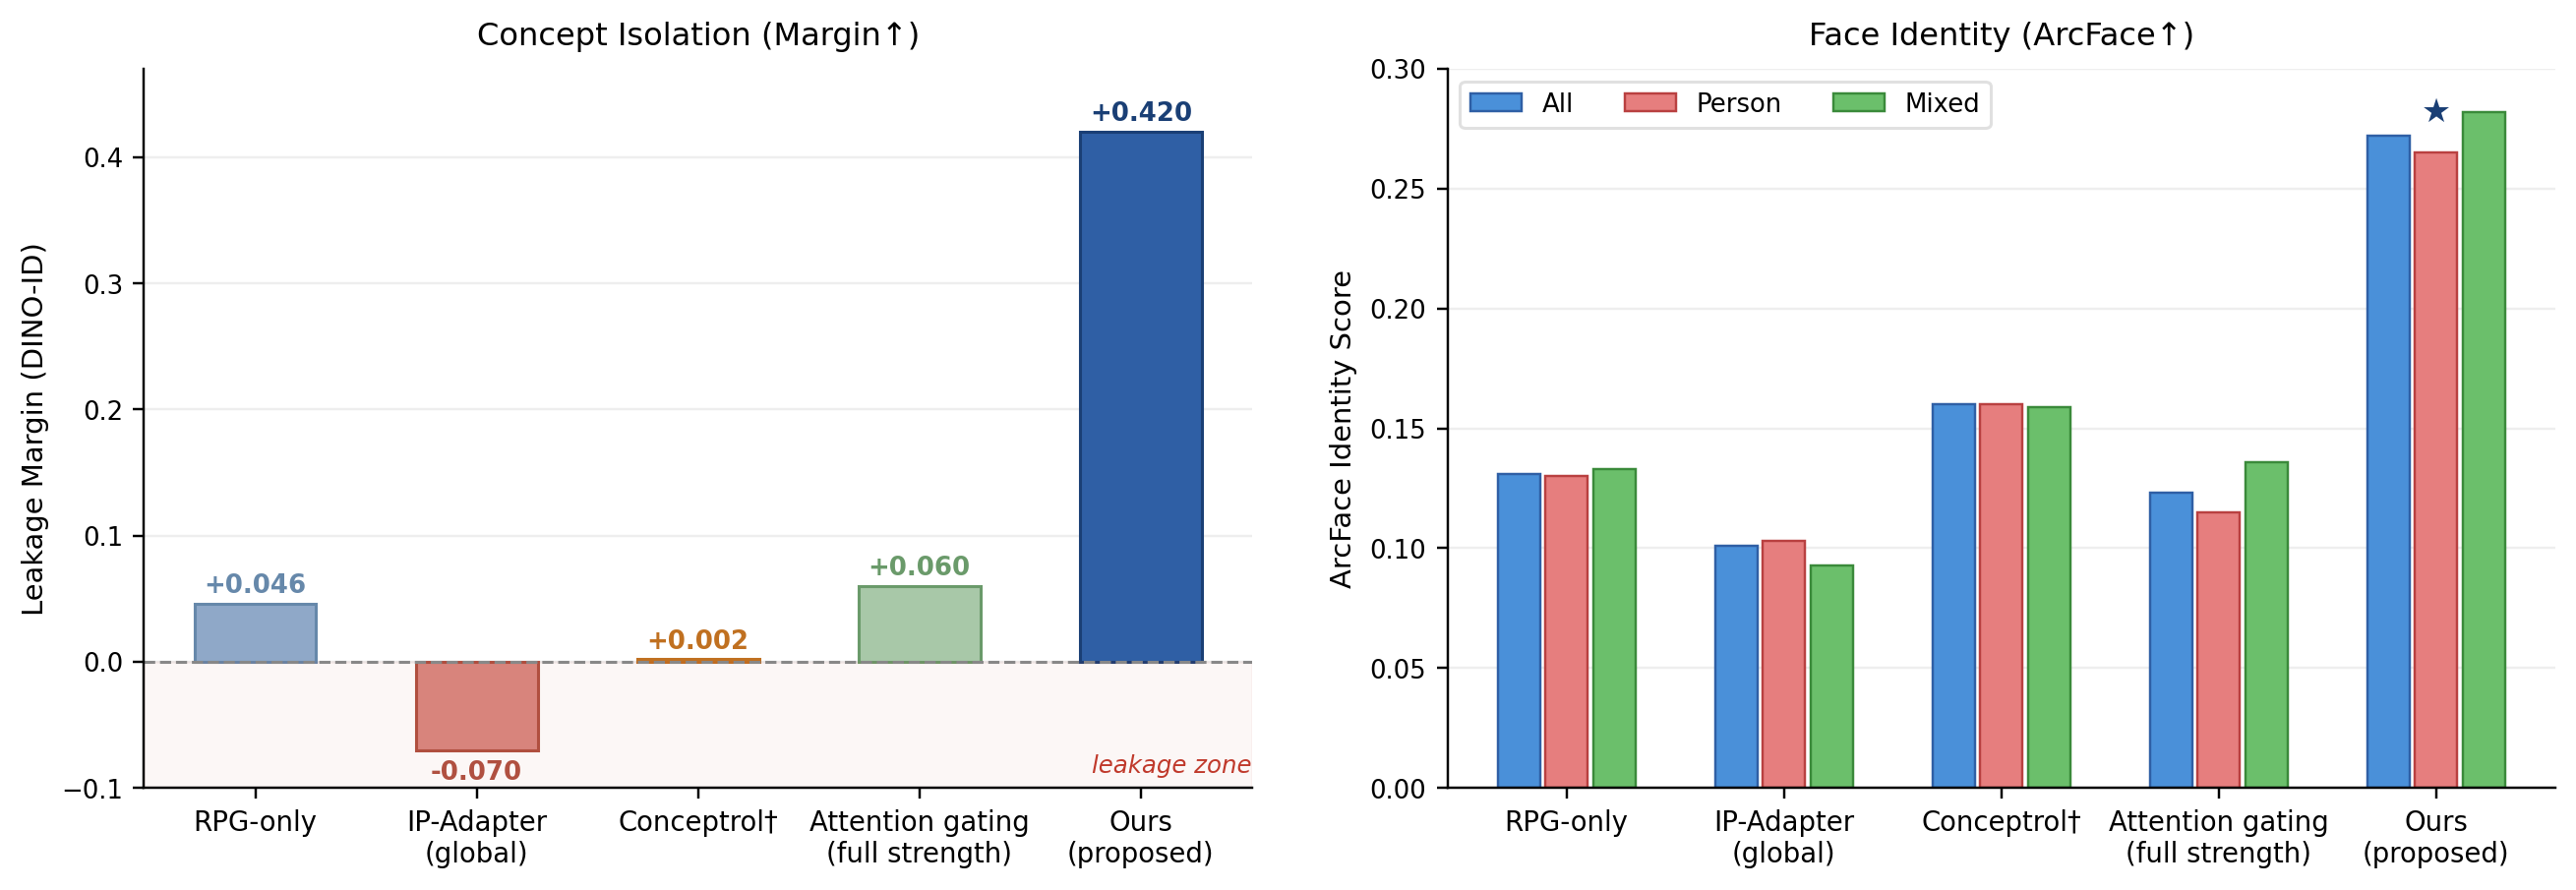
\includegraphics[width=\linewidth]{paper_figures/fig8_metrics_chart.png}
  \caption{%
    \textbf{Metric comparison.}
    Left: Leakage Margin.  Global IP-Adapter falls below zero (leakage zone,
    red shading); Conceptrol$^{\dagger}$ and attention gating at full strength
    sit at essentially zero, i.e.\ each region crop matches the wrong reference
    as well as its own; only sub-canvas compositing separates the concepts.
    Right: ArcFace identity by category.  Conceptrol transfers more face
    identity than the other baselines but, as the Margin shows, into a single
    merged subject rather than two.
  }
  \label{fig:metrics_chart}
\end{figure}

\section{Failure Case Analysis}
\label{sec:failure}

Despite strong average performance, our method exhibits recurring
failure modes that reveal the limits of training-free spatial conditioning.
We categorise the worst-performing samples (DINO-ID $< 0.16$) from
Mixed-Eval-v1 into four patterns:

\noindent\textbf{(F1) Crowded three-region layouts.}
When $N{=}3$ equal-width regions are used, each strip is only
$\sim$341\,px wide at 1024\,px resolution.
The IP-Adapter cross-attention guidance spreads across the narrow strip
and cannot fully suppress leakage from adjacent regions.
Sample \texttt{mixed\_3r\_039} (mug $\mid$ teenager $\mid$ plant)
achieves DINO-ID\,=\,0.107 and Margin\,=\,$-$0.133—the worst leakage
in the dataset.

\noindent\textbf{(F2) Visually generic objects.}
Everyday objects such as apples, mugs, and books produce nearly
identical DINOv2 embeddings across different instances.
Even when the generated image renders the correct object category,
the metric registers low identity because DINOv2 encodes instance-level
texture rather than category membership.
Samples \texttt{object\_3r\_032} and \texttt{object\_3r\_047}
(apple/watch/mug and apple/book/plant, respectively) illustrate this:
the model generates plausible objects, but the embedding comparison
yields ID $< 0.16$.

\noindent\textbf{(F3) Contradictory textual descriptions.}
Some sub-prompts assign conflicting attributes to one subject---``long black
hair'' and ``short blonde hair'' in \texttt{person\_3r\_029}, for
instance---and both the text encoder and the adapter respond with a blended
or incoherent appearance (DINO-ID\,=\,0.150).  The fault is ours rather than
the planner's: it originates in Mixed-Eval-v1's prompt construction, which
draws two attributes without excluding pairs from the same group, and affects
$11.2\%$ of person sub-prompts (Section~\ref{sec:exp}).  The planner
propagates the contradiction faithfully.  We keep these samples in every
table because removing them after the fact would be selection on the outcome,
and because the contradiction is identical for every method compared.

\noindent\textbf{(F4) Face identity in narrow person strips.}
Three-person layouts force each face into a $\sim$341\,px strip.
ArcFace detection success drops below 50\% in these cases, and even
when faces are detected, the limited spatial extent weakens the
IP-Adapter conditioning signal relative to the background.
\texttt{person\_3r\_049} achieves DINO-ID\,=\,0.150 and
Margin\,=\,$-$0.077.

These failure modes suggest that future work should focus on
adaptive region sizing guided by concept salience, and reference
denoising strategies that increase robustness to view-angle variation.

\noindent\textbf{Single-concept identity methods do not extend to this
setting.}
We ran InstantID~\cite{wang2024instantid} at $768$ before settling on the
native-resolution protocol and do not carry the row forward, but the failure
is worth one sentence because it is structural rather than incidental: the
method derives face keypoints from \emph{one} reference and applies them as a
ControlNet condition to the \emph{entire} canvas, so in a two-person layout a
single face geometry is imposed over both regions and neither crop passes
ArcFace detection on any of the 150 samples.

% ============================================================

\section{Computational Efficiency}
\label{sec:efficiency}
% ============================================================

Table~\ref{tab:timing} reports per-image denoising time and peak GPU
memory on a single NVIDIA RTX\,5080 (16\,GB) at $768\!\times\!768$, 30
DPM-Solver++ steps.  Every configuration is measured with the
\emph{identical} inline sampler, no CPU offloading, and the VAE decode
excluded, so the numbers are directly comparable and reflect the
denoising loop alone.  A single full-canvas conditioned pass---the
per-step cost of global IP-Adapter---is the natural unit of comparison;
region-planning baselines such as RPG-only and Conceptrol perform at
least one such pass plus their own regional or masking overhead.

\begin{table}[htbp]
\centering
\caption{Inference cost (RTX\,5080\,16\,GB, $768\!\times\!768$, 30
         DPM-Solver++ steps, seed 42; \texttt{time.perf\_counter}, 5
         timed runs after 2 warm-ups, identical inline sampler, no CPU
         offload, VAE decode excluded).}
\label{tab:timing}
\resizebox{\columnwidth}{!}{%
\begin{tabular}{lcc}
\toprule
Method & s\,/\,image & $\times$\,IP-global \\
\midrule
IP-Adapter (global)      & \textbf{9.46} & 1.00$\times$ \\
\textbf{Ours}            & 9.88 & 1.04$\times$ \\
MS-Diffusion             & 11.92 & 1.26$\times$ \\
RPG-only                 & 15.64 & 1.65$\times$ \\
Attention gating         & 16.00 & 1.69$\times$ \\
Conceptrol               & 17.22 & 1.82$\times$ \\
\bottomrule
\end{tabular}%
}
\end{table}

Sub-canvas compositing evaluates the UNet once per region per step, but
each pass runs on a sub-window narrower than the full canvas, so cost
grows \emph{sublinearly} in the number of regions $N$: two regions cost
$1.4\times$ a single full-canvas pass rather than $2\times$, and three
cost $2.0\times$ rather than $3\times$.  Peak memory stays flat at
$9.5$\,GB across $N$---only one sub-canvas is resident at a time and the
footprint is dominated by the fixed SDXL and adapter weights---so the
method adds concepts within the 16\,GB budget without the memory
blow-up of batching $N$ full-resolution images.

% ============================================================

\section{Comparison with Training-Based Methods}
\label{sec:training_compare}

Our method targets the \emph{zero-shot} setting: given only inference-time
reference images, it produces personalised multi-concept images without
any per-concept optimisation.
Training-based methods—DreamBooth~\cite{ruiz2023dreambooth},
Custom~Diffusion~\cite{kumari2023multi}, and
Mix-of-Show~\cite{gu2023mix}—generally achieve higher fine-grained
identity fidelity by embedding specific concepts into model weights.
However, they require per-concept (or per-concept-pair) fine-tuning
before inference, which precludes use when reference images arrive at
test time.
Table~\ref{tab:training_cost} summarises the practical trade-off.

\begin{table}[htbp]
\centering
\caption{%
  Training cost vs.\ capability comparison.
  ``Inference-time reference'' = method accepts unseen reference
  images without retraining.
  $^{*}$FreeCustom is tuning-free but additionally requires an external
  segmentation model to obtain per-concept masks.
}
\label{tab:training_cost}
\resizebox{\columnwidth}{!}{%
\begin{tabular}{lccccc}
\toprule
Method & Training & Per-concept time & Multi-concept & Inference-time ref & Backbone \\
\midrule
DreamBooth~\cite{ruiz2023dreambooth}   & Full UNet   & $\sim$30\,min & \texttimes & \texttimes & SD \\
Custom Diffusion~\cite{kumari2023multi}& Key layers  & $\sim$30\,min & Partial     & \texttimes & SD \\
Mix-of-Show~\cite{gu2023mix}           & LoRA / concept & $\sim$20\,min & \checkmark  & \texttimes & SD \\
\midrule
MC$^2$~\cite{mc2_2025}                 & Per-concept models & $\sim$20\,min & \checkmark & \texttimes & SD \\
LaTexBlend~\cite{latexblend2025}       & Per-concept bases  & $\sim$20\,min & \checkmark & \texttimes & SD \\
LoRAShop~\cite{dalva2025lorashop}      & LoRA / concept & $\sim$20\,min & \checkmark & \texttimes & Flux \\
FreeCustom~\cite{freecustom2024}       & None        & ---           & \checkmark  & \checkmark & SD\,1.5$^{*}$ \\
\midrule
MS-Diffusion~\cite{wang2025msdiffusion}& Corpus, once & \textbf{---} & \checkmark & \checkmark & SDXL \\
FastComposer~\cite{xiao2024fastcomposer}& Corpus, once & \textbf{---} & \checkmark & \checkmark & SD \\
XVerse~\cite{chen2025xverse}           & Corpus, once & \textbf{---} & \checkmark & \checkmark & Flux \\
\midrule
IP-Adapter (global)                    & None        & ---           & \checkmark  & \checkmark & SDXL \\
\textbf{Ours}                          & \textbf{None} & \textbf{---} & \checkmark  & \checkmark & SDXL \\
\bottomrule
\end{tabular}%
}
\end{table}

\noindent
The distinction that matters is not training in general but \emph{per-concept}
training.  Methods in the first block bake each concept into weights before
inference, so a reference photograph first seen at test time cannot be used at
all; quantitative comparison against them would confound the mechanism under
study with a strictly easier problem setting, and we do not attempt it.
Methods in the second block are trained once on a subject-annotated corpus and
are then zero-shot exactly as we are.  Those \emph{are} directly comparable,
and the strongest of them that targets our layout-conditioned setting on our
backbone, MS-Diffusion, is evaluated head-to-head in Table~\ref{tab:main}
under a matched protocol.  On that benchmark we lead it on identity,
placement and isolation and trail it on text alignment
(Section~\ref{sec:main_results}), and we present both halves, including the
layout convention under which the isolation result reverses.  What our method
offers besides is the absence of a subject-annotated training corpus and a
lower cost per image ($9.88$\,s against $11.92$\,s); what the comparison
establishes for the argument of this paper is that
the separation both methods achieve is unreachable by the training-free
attention-gated route, whether it is bought with supervision or with a change
of injection site.

\noindent\textit{On recent multi-concept methods.}
The 2025 multi-concept literature is dominated by two families, neither
of which yields a like-for-like baseline in our setting.
MC$^2$~\cite{mc2_2025} and LaTexBlend~\cite{latexblend2025} \emph{compose
pre-trained single-concept models}: every concept must first be embedded
into weights by a per-concept optimisation run, so they inherit the
training-based limitation above and cannot consume a reference photograph
that first appears at test time.
FreeCustom~\cite{freecustom2024} is genuinely tuning-free, but couples a
multi-reference self-attention mechanism to an SD\,1.5 backbone and
additionally requires an external segmentation network to produce the
per-concept masks it filters with; differences in backbone capacity and
mask supervision would dominate any direct metric comparison against our
SDXL pipeline.
We therefore compare against the mechanism these methods share---confining
identity \emph{inside} the attention operator---rather than against their
individual implementations, which is exactly the attention-gating ablation
of Table~\ref{tab:ablation}.  That ablation is backbone-, planner- and
seed-matched to our method, and so isolates the design choice under study
instead of conflating it with backbone differences.

% ============================================================

\section{Where the panel boundary comes from, and what closes it}
\noindent\textit{The control we should have run first, and the conclusion it
overturns.}
Nine failures spread across geometry, receptive field, and post-processing
invite the conclusion that the panel structure is intrinsic to noise-level
fusion.  An earlier draft of this analysis drew exactly that conclusion.  It
is wrong, and the control that refutes it is the cheapest one available.  We
ran the method with the same regions, the same overlap, the same schedule and
the same fusion rule, changing one thing: the adapter scale is set to zero, so
each sub-canvas is driven by its text prompt alone.  The boundary step is
$1.059$, against $1.103$ for the method as reported and $1.37$ for a collage,
on the same 30 samples.  Sub-canvas fusion applied to text-conditioned regions
leaves no visible seam.  What leaves one is the references: two photographs
taken in different places, transferred whole by the adapter---background
included---and each reproduced faithfully by the pass that receives it.  The
boundary is where two reproduced scenes meet.

This reattribution predicts its own repair, and the prediction holds.
Segmenting each subject and compositing it onto a common ground before
encoding gives the two passes nothing left to disagree about, and the step
returns to the text-only floor: $1.062$ on flat grey, $1.017$ on a shared
defocused backdrop.  The dose behaves as the account requires---blurring that
shared backdrop by $24$ pixels rather than $48$ leaves enough of the original
scene legible for the two passes to keep disagreeing, and the step stays at
$1.096$, statistically indistinguishable from the method as reported.  The
price is a small but real loss of identity, $-0.035$ and $-0.033$ DINO-ID
respectively (both $p{<}0.01$), because the discarded background was carrying
part of what DINO was matching on.

Most of that identity loss is recoverable, and the way it is recovered
confirms the mechanism a second time.  A binary silhouette composites the
subject onto the ground as a cut-out, and the adapter transfers the cut-out
edge along with the subject; blurring the segmentation alpha by $24$ pixels so
that the subject fades into the ground instead recovers two fifths of the
loss, to $-0.019$ DINO-ID and $-0.027$ Margin, while holding the step at
$1.016$.  Against the unfeathered variant the identity gain is $+0.014$
($p{=}0.046$).  The best repair we have is therefore a preprocessing step on
the references alone: segment, composite onto one defocused ground, feather
the seam.  It touches neither the fusion rule nor the layout, which is the
point.

\noindent\textit{When it works and when it cannot.}
The repair is bounded by what segmentation can extract.  Where each reference
contains a subject with a silhouette---a person, an animal, an object---the
two grounds agree and the boundary closes.  Where a reference \emph{is} a
scene, as with our stained-glass and multi-panel character-sheet references,
there is no subject to lift off it, the segmenter returns most of the frame,
and the panel survives every variant above.  That is a limitation of the
diagnosis and also a small confirmation of it: the boundary persists in
exactly the cases where the two references still carry incompatible contexts
after the repair.

Two honest qualifications.  The $1.017$ figure sits \emph{below} the
text-only floor, and it should: with the same blurred image behind both
subjects the low-frequency field is continuous by construction, so on this
one variant the measure is partly reporting what we built rather than what
was generated.  And a defocused ground is not the prompted scene---the seam
is gone, but so is the setting, which is the same trade
Section~\ref{sec:why_gating_fails} reaches from the other direction.  We
therefore report the segmented-reference variants as a diagnosis that
localises the cause and as an optional preprocessing step with a measured
price, not as a replacement for the method whose numbers this paper reports:
every comparison in Sections~\ref{sec:main_results}--\ref{sec:scaling} is run
without it, so that what is compared across methods is the generation
procedure and not our choice of segmenter.  The
two directions that would keep the scene are outside this paper's setting:
token replacement in a backbone whose tokens carry semantics, which requires
a DiT, and a trained grounding module, which requires the corpus whose
absence is the point of a training-free comparison.

\section{The frontier is the backbone's, not the tuning's}
\label{sec:architecture}

Every configuration in this study trades identity against framing, and the
trade is remarkably stable: across four mechanisms and roughly twenty
configurations, more identity arrives only with a larger face, a tighter crop
and a boundary between the regions.  Nothing we tried escaped it.  A reader is
entitled to suspect that a study which fails twenty times has simply not found
the right setting.

Concurrent work names the reason, and it is architectural rather than a matter
of search.  Feng et al.~\cite{feng2026personalize} observe that a diffusion
transformer represents content in tokens whose position is supplied separately,
so a reference's tokens can be injected \emph{without} their positional
information, whereas a U-Net's convolutions entangle content with position and
reproduce the reference's spatial arrangement along with its appearance.  Our
measurements are the U-Net side of exactly that statement.  A CLIP image
embedding fed to IP-Adapter cannot deliver ``who this is'' without also
delivering ``framed like this'': raising the adapter's strength collapses the
prompt's medium shot to the reference's bust ($9.5\% \to 20.5\%$ face area,
Table~\ref{tab:textstream}), and lowering it removes the identity instead.  The
same entanglement explains why sub-canvas compositing scores highest on
identity while sitting closest to a literal paste, and why attention gating
inside RPG recovers no identity at any strength (Table~\ref{tab:cascade}): a
spatial mask can restrict where entangled content lands, but cannot separate
what is entangled.

Read that way, the results here and the DiT results are consistent rather than
competing.  Token replacement is the rung our ladder ends on and could not
climb---on SDXL it improves every metric we report while reproducing the
reference almost exactly (Section~\ref{sec:refresponse})---and on a DiT the
same operation succeeds, with early injection for consistency and late
regularisation for flexibility~\cite{feng2026personalize}.  The regularisation
is aimed at the failure our copy-fidelity check measures.  Work that removes
the pose entanglement without changing backbone does so by training for it:
Qian et al.~\cite{qian2025canvascomposer} disentangle pose and illumination
across subjects with a cross-reference objective, which is not available to a
training-free method.

We therefore state the scope of this paper's negative results precisely.  They
are not evidence that regional personalisation is hard; they are measurements
of what a U-Net's cross-attention can and cannot be asked to do, with the size
of each cost attached.  The text-stream route of
Section~\ref{sec:textstream} is the one configuration that sidesteps the
entanglement without leaving the backbone, and it does so by not using the
image branch at all---which is also why its scope is limited to subjects whose
identity encoder was trained on faces.

\section{Protocol for the baselines in Table~1}
\noindent
$\dagger$: Conceptrol~\cite{he2025conceptrol}, run from the authors'
  official implementation (\texttt{Conceptrol\allowbreak IPAdapter\allowbreak Plus\allowbreak XL}) with the same
  SDXL backbone, IP-Adapter Plus ViT-H weights, resolution, scheduler, steps,
  CFG and seed as ours.  Injection scales $1.0$ (the authors' default) and
  $0.8$ (matched to our $\lambda$) were both run over all 150 samples and the
  stronger of the two ($0.8$) is reported; at $1.0$ the row reads
  $0.357/{+}0.004/0.621/0.155/0.153/130.8/26.8$.  Conceptrol has no layout planner,
  so it receives the global prompt, and we supply corrected per-concept token
  spans (Section~\ref{sec:conceptrol_setup}).
  $\P$: MS-Diffusion~\cite{wang2025msdiffusion}, run from the authors'
  released code and \texttt{ms\_adapter.bin} on the same SDXL-base-1.0
  backbone, at the same resolution, scheduler, steps, CFG and seed as ours,
  and driven by our planner's regions.  Four configurations were run over the
  full benchmark---injection scale $\{0.6$ (the authors' default), $0.8$
  (matched to our $\lambda)\}$ crossed with box shape $\{$our adjacent
  full-height strips, the tighter non-adjacent shape used in the authors'
  examples$\}$---and the strongest is reported (scale $0.8$, tight boxes).
  The box shape matters more than the scale: with our strips the same scale
  reads $0.509/{+}0.327/0.645/0.215/0.212/128.9/23.8$, so passing the layout
  in the authors' own convention is worth $+0.112$ Margin to the baseline.
  Ours = the noise-fusion operating point: sub-canvas regional compositing
  with per-region full-strength
  IP-Adapter and late global release at the default $\tau{=}0.7$
  (Section~\ref{sec:tau}).
  $\ddagger$: IP-Adapter FaceID PlusV2~\cite{ye2023ip}, conditioned globally
  on the first reference of each sample---its ArcFace identity embedding
  together with the CLIP ViT-H features---at the same resolution, scheduler,
  steps, CFG and seed as ours, at the stronger of the two injection scales we
  ran ($0.6$).  In 81 of the 150 samples the guiding reference contains no
  detectable face, since the object category is not faces, so the identity
  embedding degenerates to a zero vector and only the CLIP branch remains
  active; its DINO-ID lands \emph{below} the text-only baseline as a result.
  This is inherent to applying a face-specific method to a benchmark that
  contains objects, and we report it rather than dropping the row.
  InstantID, which appeared in an earlier $768$ version of this table, is
  dropped rather than carried over at a resolution it was not re-run at; it
  scored far below every row above on every axis.

% ============================================================
\bibliographystyle{elsarticle-num}
\bibliography{refs}

\end{document}
